\documentclass[12pt,a4paper]{article}

\usepackage[spanish,es-noshorthands,es-tabla]{babel}
\usepackage[utf8]{inputenc}
\usepackage[T1]{fontenc}
\usepackage{lmodern}
\usepackage{microtype}
\usepackage{geometry}
\usepackage{setspace}
\usepackage{amsmath,amssymb}
\usepackage{booktabs}
\usepackage{tabularx}
\usepackage{longtable}
\usepackage{array}
\usepackage{enumitem}
\usepackage{xcolor}
\usepackage{graphicx}
\usepackage{float}
\usepackage{caption}
\usepackage{subcaption}
\usepackage{listings}
\usepackage{csquotes}
\usepackage[round,authoryear]{natbib}
\usepackage{hyperref}

\geometry{margin=2.5cm}
\onehalfspacing
\setlist[itemize]{leftmargin=1.4em,itemsep=0.2em,topsep=0.2em}
\setlist[enumerate]{leftmargin=1.6em,itemsep=0.2em,topsep=0.2em}
\setlength{\parskip}{0.45em}
\setlength{\parindent}{0pt}
\captionsetup{font=small,labelfont=bf}
\graphicspath{{figuras/}}

\hypersetup{colorlinks=true,linkcolor=black,citecolor=black,urlcolor=blue}

% --- colores y estilo de código (Tableau / pandas) ---
\definecolor{codbg}{HTML}{F5F5F2}
\definecolor{codkw}{HTML}{2A78D6}
\definecolor{codcm}{HTML}{6E6D68}
\definecolor{codst}{HTML}{008300}
\definecolor{acento}{HTML}{4A3AA7}
\lstdefinestyle{cod}{
  backgroundcolor=\color{codbg}, basicstyle=\ttfamily\footnotesize,
  keywordstyle=\color{codkw}\bfseries, commentstyle=\color{codcm}\itshape,
  stringstyle=\color{codst}, breaklines=true, showstringspaces=false,
  columns=fullflexible, frame=leftline, framerule=1.2pt, rulecolor=\color{acento},
  xleftmargin=0.8em, framexleftmargin=0.8em, aboveskip=0.7em, belowskip=0.5em,
  morekeywords={FIXED,TOTAL,SUM,AVG,MEDIAN,PERCENTILE,WINDOW_AVG,RUNNING_SUM,
  LOOKUP,RANK,CORR,ZN,IIF,CASE,WHEN,THEN,ELSE,END}
}
\lstset{style=cod}

% --- comando para la bitácora (protocolo de la pregunta 4) ---
\newcommand{\bitacora}[5]{%
\begin{enumerate}[label=\textbf{\arabic*.},leftmargin=1.8em]
  \item \textbf{Lectura inicial:} #1
  \item \textbf{KPI decisor:} #2
  \item \textbf{Giro analítico:} #3
  \item \textbf{Lectura revisada:} #4
  \item \textbf{Consecuencia:} #5
\end{enumerate}}

\begin{document}

% ======================= CARÁTULA =======================
\begin{titlepage}
\centering
\vspace*{1.4cm}
\IfFileExists{upc-logo.png}{
\includegraphics[width=3.2cm]{upc-logo.png}\\[1cm]}{\vspace{1cm}}
{\Large\textbf{UNIVERSIDAD PERUANA DE CIENCIAS APLICADAS}}\\[0.3cm]
{\large Facultad de Ingeniería}\\
{\large Ciencia de la Computación}\\[1.6cm]
{\large\textbf{Visualización de Datos}}\\
{\large Examen Final}\\[1.6cm]
{\LARGE\textbf{Operación ChasquiFest}}\\[0.35cm]
{\Large auditoría de visualización de cinco casos}\\[0.6cm]
{\large\itshape Qué se puede afirmar, cómo debe medirse y qué gráfico permite decidir}\\[2.2cm]
\textbf{Estudiante:}\\
Rody Sebastian Vilchez Marin (U202216562)\\[1.4cm]
\vfill
Lima, Perú\\
2026
\end{titlepage}

\tableofcontents
\newpage

% ======================= INTRODUCCIÓN =======================
\section{Introducción}

ChasquiFest es una gira cultural ficticia que llevó música, gastronomía, diseño y tecnología a doce sedes del Perú. Killa, la llama-mascota, se volvió viral; el patrocinador ya mandó imprimir un cartel que dice \emph{éxito histórico} y el comité directivo se reúne en dos horas. El problema es que el \emph{workbook} que sustenta esa afirmación mezcla porcentajes no aditivos, escalas distorsionadas, ventanas temporales no homólogas y conclusiones causales extraídas de asociaciones observacionales.

Este informe adopta el rol de \textbf{auditoría visual}. Para cada uno de cinco casos se toma un gráfico engañoso del tablero original y se decide, con evidencia recalculada desde los datos, qué se puede afirmar, cómo debe medirse el indicador y qué visualización permite tomar la decisión sin convertir una correlación simpática en una ley de la naturaleza. La tesis transversal es simple: en analítica de decisión, \emph{el denominador, la ventana temporal y el canal perceptual eligen la conclusión tanto como el dato} \citep{cleveland1984graphical,tufte2001visual}.

Todo el festival, sus personajes y sus cifras son \textbf{ficticios y sintéticos}. Los nombres geográficos se usan para dar contexto peruano; los datos no describen el desempeño real de ninguna ciudad ni población.

% ======================= METODOLOGÍA =======================
\section{Metodología}

\subsection{Datos y herramientas}
El material son cinco archivos CSV sintéticos, uno por caso, con granularidad declarada distinta (una fila por evento$\times$canal en el Caso~1; por envío en el Caso~2; por mes$\times$sede en el Caso~3; por sede en el Caso~4; por fecha$\times$sede en el Caso~5). Todo cálculo se recomputa desde el CSV con \texttt{pandas}; las figuras se generan con \texttt{matplotlib} sobre una hoja de estilo común (tipografía serif, paleta \emph{colorblind-safe} validada, ejes recesivos y salida vectorial). Donde el examen pide una fórmula de Tableau se ofrece la sintaxis Tableau y su símil en código. El proyecto es reproducible: notebooks ejecutables por caso y datos acompañan a este informe.\footnote{Repositorio y notebooks: \url{https://github.com/R0SEWT/chasquifest-auditoria-visual}}

\subsection{Regla de auditoría y criterios de calidad}
Cada respuesta se construye con cuatro piezas cuando corresponden: (1)~el \textbf{concepto técnico}; (2)~la \textbf{evidencia} con campos y números concretos del dataset; (3)~la \textbf{decisión} de cálculo o de diseño; y (4)~un \textbf{límite} o \emph{trade-off}. Además, el informe se somete a seis criterios de rigor que funcionan como controles de calidad:

\begin{itemize}
  \item Todo porcentaje declara \textbf{numerador y denominador}.
  \item Toda recomendación de gráfico nombra la \textbf{tarea analítica} (comparar, correlacionar, ver distribución, \emph{ranking}, parte-todo, tendencia, localización).
  \item Toda \emph{table calculation} declara \textbf{partición} y \emph{addressing}.
  \item Ninguna comparación entre periodos se hace sin verificar \textbf{homologación}.
  \item Ninguna \textbf{causalidad} se afirma a partir de asociación observacional \citep{simpson1951interpretation,anscombe1973graphs}.
  \item Todo KPI se presenta con \textbf{periodo, comparación/meta y decisión} asociada.
\end{itemize}

La pregunta~4 de cada caso cierra con una \textbf{bitácora} de cinco frases (lectura inicial, KPI decisor, giro analítico, lectura revisada y consecuencia) que documenta explícitamente qué evidencia obligó a abandonar o matizar la primera interpretación.

% ======================= CASOS =======================
\section{Caso 1 --- La torta porcentual que nadie pidió}\label{sec:caso1}

El tablero original de taquilla arma una torta de \enquote{participación en el éxito} con tres porciones: App~35.7\%, Web~33.8\% y Taquilla~30.5\%. Nadie en la reunión logra decir a qué total se refiere ese 35.7\%, y la razón es sencilla: no se refiere a ningún total. El practicante tomó \lstinline|ocupacion_fila_pct|, un ratio que ya viene calculado \emph{por fila} (\lstinline|evento_id|~$\times$~\lstinline|canal|, $n=216$ filas), y lo \textbf{sumó} por canal para trazar la torta. El denominador de esa torta es \enquote{la suma de 216 porcentajes de fila}, una cantidad sin significado de negocio: la suma de ratios no es el ratio de las sumas. Antes de continuar se verificó, recalculando directamente desde el CSV, que en efecto \lstinline|ocupacion_fila_pct| $=$ \lstinline|ingresos_validados|/\lstinline|cupos_ofertados|$\times 100$ (diferencia máxima $0.0049$ pp) y que \lstinline|margen_fila_pct| $=$ (\lstinline|ventas_soles|$-$\lstinline|costo_variable_soles|)/\lstinline|ventas_soles|$\times 100$ (diferencia máxima $0.0050$ pp): ambas son fórmulas de fila, no aditivas entre sí.

\subsection{Pregunta 1 --- Promedio de promedios}\label{ssec:c1-q1}

\paragraph{Concepto técnico.} Existen dos maneras de agregar una columna que ya es un ratio. La primera es \emph{ratio-of-sums}: se suman numerador y denominador por separado en todo el universo deseado y se divide al final, con lo cual cada fila pesa según su tamaño real.
\[
\text{Ocupación ponderada} = \frac{\sum \text{ingresos\_validados}}{\sum \text{cupos\_ofertados}} \times 100
\]
La segunda es \emph{mean-of-ratios}: se promedian los ratios de fila ya calculados, dando el mismo peso (un voto) a una fila de 521 cupos que a una de 4\,812 cupos.
\[
\text{Ocupación promedio simple} = \operatorname{AVG}(\text{ocupacion\_fila\_pct})
\]
\lstinline|AVG([ocupacion_fila_pct])| responde \enquote{¿cuál es el ratio promedio de una fila evento-canal cualquiera?}, no \enquote{¿qué fracción de la capacidad total del festival se ocupó?}. La pregunta de negocio de la jefa de taquilla es de \textbf{capacidad total}, y solo el ratio-of-sums la responde correctamente.

\paragraph{Evidencia.} Ocupación ponderada $=$ SUM(\lstinline|ingresos_validados|)/SUM(\lstinline|cupos_ofertados|)$\times 100 = 281\,091/311\,400\times 100 = 90.27\%$. Ocupación promedio simple $=$ AVG(\lstinline|ocupacion_fila_pct|) sobre $n=216$ filas $= 88.17\%$. La meta, tomada de la columna \lstinline|meta_ocupacion_pct| (valor único en todo el CSV), es $88.0\%$. A nivel de temporada completa ($N=216$, grano homogéneo evento$\times$canal) \textbf{ambas métricas superan la meta}, pero con colchones muy distintos: $+2.27$ pp la ponderada frente a $+0.17$ pp la promedio simple — la lectura ponderada dice \enquote{cumplida con holgura}, la no ponderada dice \enquote{cumplida raspando, un evento chico y flojo la tumba}. Al cortar por mes sí aparece una divergencia de signo: en julio 2026 la ponderada da $89.91\%$ (CUMPLE) y la promedio simple da $87.14\%$ (\textbf{NO CUMPLE}) — evidencia directa de que ambos estimadores pueden decidir distinto frente a la misma meta. Advertencia adicional de homologación: los 12 eventos de julio-2026 están fechados el 25-jul-2026 y los 12 de agosto también son posteriores a \enquote{hoy} (18-jul-2026, fecha de contexto del examen); el CSV ya trae \lstinline|ingresos_validados| cargado para esas filas, de modo que se trata de una temporada completa pre-cargada para el ejercicio, no de un feed operativo en vivo. El corte mensual aquí solo sirve para \emph{ilustrar} que el promedio simple y la razón ponderada pueden discrepar; el KPI oficial de temporada debe reportarse a nivel global ($N=216$).

\paragraph{Decisión.} Fórmula agregada (Tableau, ratio-of-sums):
\begin{lstlisting}[style=cod]
Ocupacion Global % =
SUM([ingresos_validados]) / SUM([cupos_ofertados])
\end{lstlisting}
símil en \lstinline|pandas|:
\begin{lstlisting}[style=cod]
occ_weighted = df['ingresos_validados'].sum() / df['cupos_ofertados'].sum() * 100
\end{lstlisting}
Lo que \textbf{no} debe usarse (el espíritu del error del practicante, aplicado a ocupación):
\begin{lstlisting}[style=cod]
AVG([ocupacion_fila_pct])          -- Tableau, mean-of-ratios, sesgado
df['ocupacion_fila_pct'].mean()    -- pandas, mismo sesgo
\end{lstlisting}
La Figura~\ref{fig:c1-q1} presenta ambos estimadores del mismo KPI junto a la línea de meta: cruzan la meta con colchones distintos y, a corte mensual, incluso con veredictos opuestos.

\begin{figure}[H]
\centering
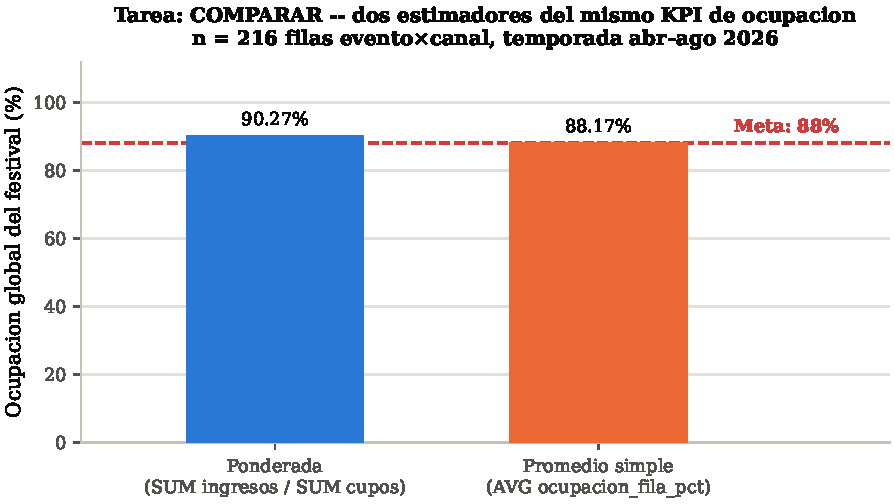
\includegraphics[width=0.85\linewidth]{caso1_q1_ocupacion.pdf}
\caption{Tarea comparar: ocupación global ponderada (ratio-of-sums, $90.27\%$) frente a la promedio simple de \lstinline|ocupacion_fila_pct| (mean-of-ratios, $88.17\%$), con la meta de $88\%$ como referencia.}
\label{fig:c1-q1}
\end{figure}

\paragraph{Límite / trade-off.} El ratio-of-sums exige que numerador y denominador estén en la misma unidad y grano que la pregunta de negocio (aquí, personas y cupos, directamente sumables); no sirve para razones que no son sumables sin más contexto (por ejemplo, promediar tasas ya normalizadas por tamaños muy heterogéneos, como un NPS por evento). La ponderada, además, oculta la varianza entre filas: un festival puede mostrar $90.27\%$ ponderado y aun así tener una fila puntual muy floja (véase Taquilla, Pregunta~2), de modo que conviene reportar ambas cifras junto con la dispersión, no solo la ponderada. Y como se advirtió arriba, todo corte temporal debe declarar explícitamente si compara eventos ya realizados contra eventos programados \citep{gelman2007average}.

\subsection{Pregunta 2 --- Nivel del cálculo}\label{ssec:c1-q2}

\paragraph{Concepto técnico.} \lstinline|ocupacion_fila_pct| y \lstinline|margen_fila_pct| son \textbf{row-level}: una fórmula evaluada por cada fila \lstinline|evento_id|$\times$\lstinline|canal|, no aditiva entre filas. Ocupación global, margen global y ticket promedio son \textbf{medidas agregadas}, que solo tienen sentido calculadas como ratio-of-sums en el grano deseado (festival, canal, departamento o periodo) — nunca como \lstinline|AVG()| de una columna row-level ya calculada.

\paragraph{Evidencia.} Margen global: num $=$ SUM(\lstinline|ventas_soles|)$-$SUM(\lstinline|costo_variable_soles|) $= 5\,949\,746.23$; den $=$ SUM(\lstinline|ventas_soles|) $=10\,473\,741.35$ $\Rightarrow$ margen ponderado $=56.81\%$, frente a $57.33\%$ de promedio simple de \lstinline|margen_fila_pct| ($n=216$) — la misma disyuntiva ratio-of-sums vs mean-of-ratios de la Pregunta~1, aquí con una distorsión leve ($0.52$ pp) porque el tamaño de fila es más homogéneo que en ocupación (donde la distorsión fue $2.10$ pp, porque \lstinline|cupos_ofertados| varía más entre canales: App/Web $\sim 2\,700$--$4\,800$ frente a Taquilla $\sim 1\,800$--$1\,925$). El sesgo de tamaño crece con la heterogeneidad del denominador. Ticket promedio por orden: num $=$ SUM(\lstinline|ventas_soles|) $=10\,473\,741.35$; den $=$ SUM(\lstinline|ordenes|) $=140\,308$ $\Rightarrow$ S/~$74.65$ por orden. No hay filas con denominador cero en cupos, ventas ni órdenes, pero la protección se declara igual como buena práctica. Ambos KPI se calculan sobre la temporada completa abr--ago~2026 ($N=216$ filas / 72 eventos); el CSV no trae meta externa de margen ni de ticket, por lo que el benchmark interno es la mediana entre canales: margen $56.56\%$ (App $56.18\%$, Web $56.56\%$, Taquilla $59.20\%$) y ticket S/~$73.26$ (App S/~$78.72$, Web S/~$73.26$, Taquilla S/~$66.04$). El margen global ($56.81\%$) queda apenas $0.25$ pp sobre esa mediana y muy cerca del margen de App ($56.18\%$, el canal de mayor volumen), señal de que el global es \enquote{jalado} hacia abajo por el peso de App; conviene revisar la mezcla de canales antes de tocar precio o comisión. El ticket global (S/~$74.65$) queda ligeramente sobre la mediana por el mismo arrastre de App; Taquilla combina el ticket más bajo (S/~$66.04$) con el margen más alto ($59.20\%$), lo que sugiere margen para una política de precio diferenciada sin erosionar su rentabilidad.

\paragraph{Decisión.} Margen global (Tableau, protegido contra división por cero):
\begin{lstlisting}[style=cod]
Margen Global % =
IIF(SUM([ventas_soles]) = 0, NULL,
    (SUM([ventas_soles]) - SUM([costo_variable_soles])) / SUM([ventas_soles]))
\end{lstlisting}
Ticket promedio:
\begin{lstlisting}[style=cod]
Ticket Promedio =
IIF(SUM([ordenes]) = 0, NULL, SUM([ventas_soles]) / SUM([ordenes]))
\end{lstlisting}
Nota sobre \lstinline|ZN()|: en Tableau solo convierte \lstinline|NULL| en $0$ (protege agregaciones de nulos), \textbf{no} protege contra división por cero; para eso se necesita \lstinline|IIF(denominador=0, NULL, ...)| como arriba. Usar \lstinline|ZN()| únicamente en el denominador de una división puede convertir un \lstinline|NULL| válido en $0$ y producir un error real de división por cero. Clasificación de negocio de los tres KPI: \textbf{Ocupación (guardrail)} — \lstinline|cupos_ofertados| es un tope físico/contractual por sede-canal-evento y la meta $88\%$ es un piso operativo pactado, no un objetivo de rentabilidad; no puede superar el $100\%$ y operar muy por debajo desperdicia capacidad ya comprometida con la sede. \textbf{Margen (resultado)} — mide directamente la rentabilidad de cada canal-evento tras costo variable, el resultado financiero que en última instancia interesa a la organización. \textbf{Ticket promedio (eficiencia)} — mide cuánto valor se extrae por transacción, proxy de mezcla de precio/tamaño de compra; es un indicador de productividad comercial, ni resultado final ni límite duro de capacidad.

La Figura~\ref{fig:c1-q2} compara margen y ocupación ponderados por canal: \textbf{Taquilla} tiene el mayor margen ($59.20\%$) pero la menor ocupación ($81.15\%$); \textbf{App} tiene la mayor ocupación ($94.51\%$) con margen algo menor ($56.18\%$) — ambos KPI no se mueven juntos.

\begin{figure}[H]
\centering
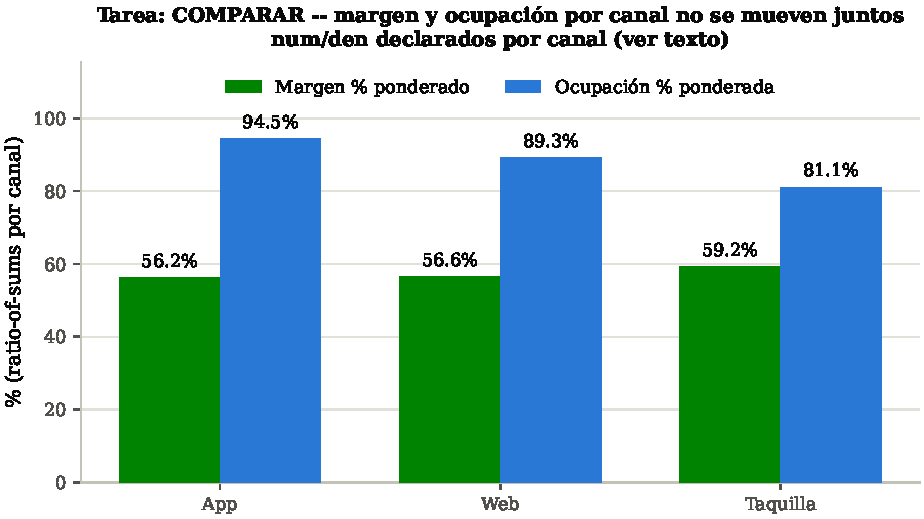
\includegraphics[width=0.85\linewidth]{caso1_q2_metricas_canal.pdf}
\caption{Tarea comparar: margen \% y ocupación \% ponderados por canal (ratio-of-sums en cada caso). Taquilla domina en margen y App en ocupación.}
\label{fig:c1-q2}
\end{figure}

Por qué mejorar un KPI no garantiza mejorar los otros, con evidencia del propio CSV (asociación, no causalidad): la correlación entre \lstinline|ocupacion_fila_pct| y \lstinline|margen_fila_pct| ($n=216$ filas) es $r=-0.43$ — asociación negativa moderada, consistente con la intuición del enunciado (\enquote{descuento sube ocupación pero baja margen}), aunque no probada causalmente aquí; un confusor plausible es el propio canal (Taquilla concentra mayor margen con menor ocupación; App, lo inverso, probablemente por comisiones de plataforma o descuentos digitales que Taquilla física no paga). La correlación entre ticket y ocupación es $r=+0.42$ (positiva, moderada), que \textbf{contradice} la intuición ingenua de \enquote{precio alto ahuyenta demanda} citada en el enunciado: en este CSV el canal con mayor ticket (App, S/~$78.72$) es también el de mayor ocupación ponderada ($94.51\%$), probablemente confundido por el canal mismo. Entre ticket y margen la correlación es débil ($r=-0.16$); Taquilla es un valor atípico que domina el signo y, controlando por canal, la relación podría invertirse o desaparecer.

\paragraph{Límite / trade-off.} Ninguna correlación aquí prueba causalidad: son asociaciones a nivel evento-canal con canal, sede y estacionalidad como confusores no controlados \citep{simpson1951interpretation}. Antes de tomar una decisión de \emph{pricing} o descuento basada en \enquote{subir ocupación baja margen} se necesitaría un diseño que aísle el efecto del canal (por ejemplo, comparar el mismo canal en eventos con y sin promoción) en vez de comparar canales estructuralmente distintos entre sí.

\subsection{Pregunta 3 --- LOD, total visible y filtros}\label{ssec:c1-q3}

\paragraph{Concepto técnico.} Existen dos formas de calcular \enquote{participación del canal dentro de su departamento} que usan denominadores con reglas de filtrado distintas. \lstinline|{ FIXED [departamento] : SUM([ventas_soles]) }| es una expresión de nivel de detalle (LOD) \emph{fija}: calcula el total de ventas del departamento ignorando los filtros de dimensión de la hoja (fecha, canal, etc.), porque en el orden de operaciones de Tableau los filtros de dimensión normales se aplican \emph{después} de las LOD FIXED; solo un filtro de contexto se evalúa antes y sí recorta lo que ve el FIXED. \lstinline|TOTAL(SUM([ventas_soles]))| es una \emph{table calculation}: sí respeta los filtros de dimensión, porque se calcula sobre las marcas que ya quedaron en el panel después de filtrar. Declaración obligatoria de partición y \emph{addressing}: en una vista con \lstinline|departamento| en filas/paneles y \lstinline|canal| en columnas dentro de cada panel, \lstinline|TOTAL(SUM([ventas_soles]))| debe direccionarse (\emph{addressing}) por \lstinline|canal| y particionarse por \lstinline|departamento| — recalcula recorriendo las marcas de canal dentro de cada panel de departamento por separado. Si \lstinline|departamento| no se declara como partición, \lstinline|TOTAL()| sumaría canal y departamento juntos, devolviendo el gran total del festival en vez del total por departamento.

\paragraph{Evidencia.} La participación de cada canal dentro de su propio departamento (12 departamentos; num $=$ SUM ventas canal-departamento, den $=$ SUM ventas departamento) es muy estable: App oscila entre $53.08\%$ (Junín) y $54.55\%$ (Ayacucho); Web entre $28.37\%$ (Ucayali) y $30.27\%$ (Lambayeque); Taquilla entre $16.28\%$ (Ayacucho) y $18.04\%$ (Junín) — coherente con el share nacional (App~$53.7\%$, Web~$29.3\%$, Taquilla~$17.0\%$; num $=$ SUM ventas canal, den $=$ SUM ventas total $=$ S/~$10\,473\,741.35$). Como ejemplo de FIXED vs TOTAL de panel visible, para el departamento Lima, canal App: \textbf{FIXED} (histórico completo, 6 eventos) $\Rightarrow$ num $=$ S/~$987\,279.17$, den $=$ S/~$1\,823\,558.36$ $\Rightarrow$ $54.14\%$; \textbf{TOTAL de panel visible} (solo eventos con \lstinline|fecha_evento| $<$ 18-jul-2026, 4 eventos, filtro de fecha como filtro de dimensión) $\Rightarrow$ num $=$ S/~$682\,899.45$, den $=$ S/~$1\,278\,780.13$ $\Rightarrow$ $53.40\%$. Los denominadores difieren (S/~$1\,823\,558.36$ frente a S/~$1\,278\,780.13$) porque miden universos distintos (6 eventos frente a 4): los porcentajes $54.14\%$ y $53.40\%$ no se contradicen, describen preguntas distintas.

\paragraph{Decisión.} El tablero debe ofrecer dos medidas en paralelo, cada una con su título aclaratorio. \emph{Participación histórica del canal en el departamento} usa FIXED como denominador y no se mueve aunque el usuario cambie el filtro de fecha, salvo que ese filtro se convierta en filtro de contexto (el contexto se evalúa antes que la LOD). \emph{Participación dentro del periodo visible} usa TOTAL() como denominador y se recalcula cada vez que el usuario mueve el filtro de fecha o de canal. Titulares válidos que no se contradicen: con FIXED, \enquote{App concentra $\sim 54\%$ de las ventas históricas de Lima (temporada completa, 6 eventos)}; con TOTAL(), \enquote{En lo que va de la temporada (4 eventos ya realizados al 18-jul-2026), App representa $53.4\%$ de las ventas visibles de Lima}. Símil en \lstinline|pandas|:
\begin{lstlisting}[style=cod]
# FIXED -> ignora cualquier filtro de dimension posterior
df['ventas_depto_FIXED'] = df.groupby('departamento')['ventas_soles'].transform('sum')

# TOTAL() del panel visible -> se recalcula DESPUES de aplicar el filtro
visible = df[df['fecha_evento'] < '2026-07-18']
visible['ventas_depto_TOTAL'] = visible.groupby('departamento')['ventas_soles'].transform('sum')
\end{lstlisting}

La Figura~\ref{fig:c1-q3} sustituye la torta falsa por la tarea parte-todo correcta y, además, expone lado a lado el artefacto original (\enquote{torta de \%} sin denominador real) contra el share real de ventas: el orden de dominancia cambia por completo.

\begin{figure}[H]
\centering
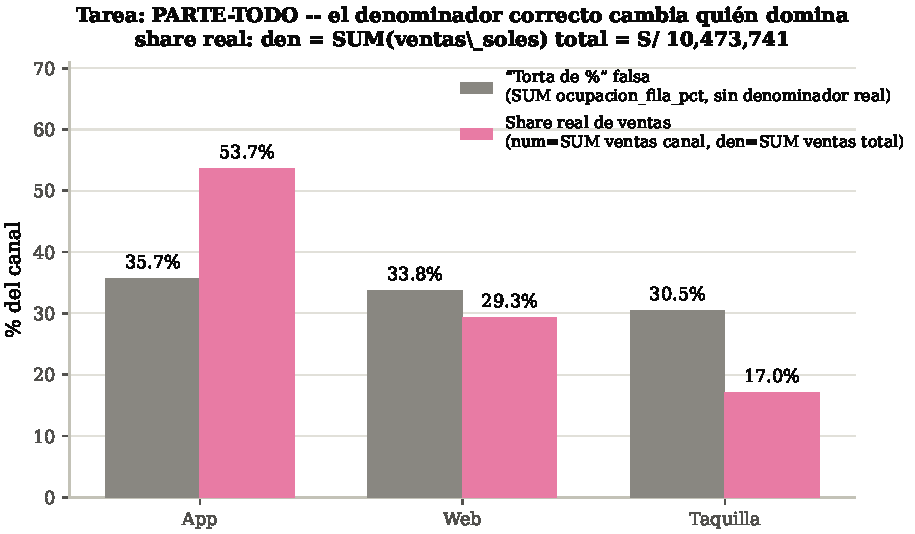
\includegraphics[width=0.85\linewidth]{caso1_q3_share.pdf}
\caption{Tarea parte-todo: \enquote{torta de \%} original (suma de \lstinline|ocupacion_fila_pct| por canal, sin denominador de negocio) frente al share real de ventas (num $=$ SUM \lstinline|ventas_soles| canal, den $=$ SUM \lstinline|ventas_soles| total). App pasa de \enquote{empatado} con los otros dos canales a dominar con más de la mitad de las ventas; Taquilla, de \enquote{casi un tercio} a apenas $17\%$.}
\label{fig:c1-q3}
\end{figure}

\paragraph{Límite / trade-off.} Convertir \lstinline|fecha_evento| o \lstinline|canal| en filtro de contexto para que también recorte el FIXED tiene costo de rendimiento (Tableau materializa una tabla temporal por cada combinación de contexto) y cambia semánticamente la pregunta: el \enquote{histórico completo} deja de existir si todo se vuelve contexto. Se recomienda dejar un único selector de fecha como filtro normal de dimensión (alimenta TOTAL/panel visible) y no tocar el filtro de contexto salvo que el usuario pida explícitamente \enquote{recalcular también el histórico}; de lo contrario los dos titulares dejan de ser comparables entre sí. La torta original se descarta en favor de la barra: con solo tres categorías la barra ordenada permite comparar magnitudes por longitud (más precisa que ángulo o área) y deja espacio para anotar el valor exacto \citep{tufte2001visual,cleveland1984graphical}.

\subsection{Pregunta 4 --- Parámetro no es filtro}\label{ssec:c1-q4}

\paragraph{Concepto técnico.} Un \textbf{filtro} decide qué filas entran al cálculo (subconjunta los datos); un \textbf{parámetro} decide cómo se calcula o se dibuja algo, sin quitar ninguna fila — es una variable global referenciada dentro de un campo calculado que afecta a toda la vista de manera consistente. Si un control debe cambiar el eje o la medida mostrada, o un umbral de comparación, sin alterar qué datos entran, debe ser parámetro; si debe excluir datos (un canal, un rango de fechas, un departamento), debe ser filtro (o filtro de contexto si además debe recortar una LOD FIXED, ver Pregunta~3).

\paragraph{Decisión.} Parámetro selector de medida, \lstinline|Medida Seleccionada| (string, lista \lstinline|Ventas|/\lstinline|Ocupación|/\lstinline|Margen|), referenciado en un campo calculado:
\begin{lstlisting}[style=cod]
Medida (segun parametro) =
CASE [Medida Seleccionada]
WHEN 'Ventas'     THEN SUM([ventas_soles])
WHEN 'Ocupacion'  THEN SUM([ingresos_validados]) / SUM([cupos_ofertados]) * 100
WHEN 'Margen'     THEN (SUM([ventas_soles]) - SUM([costo_variable_soles])) / SUM([ventas_soles]) * 100
END
\end{lstlisting}
Parámetro numérico de meta, \lstinline|Meta Ocupación %| (float, default $88$, rango sugerido $70$--$100$):
\begin{lstlisting}[style=cod]
Cumple Meta? = SUM([ingresos_validados])/SUM([cupos_ofertados])*100 >= [Meta Ocupacion %]
\end{lstlisting}
Evidencia anclada: con \lstinline|meta = 88| y la ocupación ponderada global calculada en la Pregunta~1 ($90.27\%$), el semáforo evalúa $90.27 \geq 88 \to$ \textsc{true} $\to$ CUMPLE (colchón $+2.27$ pp). Si el usuario mueve el parámetro a, por ejemplo, $92\%$, el mismo cálculo cambia a NO CUMPLE ($90.27 < 92$) sin quitar ni una fila de datos: esa invariancia del $N$ es la prueba de que se trata de un parámetro y no de un filtro.

\begin{table}[H]
\centering\small
\begin{tabularx}{\linewidth}{lll}
\toprule
Control & Tipo & Por qué \\
\midrule
Ventas / Ocupación / Margen (medida a graficar) & Parámetro & cambia el cálculo del eje, no quita filas \\
Meta de ocupación ($88\%$) & Parámetro & mueve una línea de referencia y recalcula un semáforo, no filtra \\
\lstinline|canal| (para explorar subconjuntos) & Filtro (o de contexto si alimenta un FIXED) & excluye filas \\
\lstinline|fecha_evento| / rango de fechas & Filtro (dimensión o contexto, ver P3) & excluye filas \\
\lstinline|departamento| & Filtro & excluye filas \\
\bottomrule
\end{tabularx}
\caption{Checklist parámetro vs.\ filtro para los controles del caso.}
\end{table}

Línea de referencia: en Tableau, \lstinline|Analysis > Reference Line > Add Reference Line|, tipo \emph{Constant}, valor \lstinline|[Meta Ocupación %]| (directamente el parámetro, o vía un campo calculado auxiliar si la versión lo requiere), con etiqueta \lstinline|"Meta: " + STR([Meta Ocupación %]) + "%"|. Así, cuando el usuario cambia el parámetro (p.~ej. de $88\%$ a $90\%$ para escenarios más exigentes), la línea y el semáforo se recalculan solos, sin tocar ningún filtro ni perder filas — el mismo patrón que la Figura~\ref{fig:c1-q1} de la Pregunta~1.

\paragraph{Límite / trade-off.} \lstinline|ventas_soles| (rango aproximado S/~$12\,000$--$200\,000$ por fila) y \lstinline|margen_fila_pct| u \lstinline|ocupacion_fila_pct| (rango $0$--$100$) no deben compartir un eje sincronizado: si se sincronizan, una barra en soles aplastaría visualmente la línea de porcentaje (o viceversa) y la altura de las marcas dejaría de representar la magnitud real de cada serie. Si se usa \emph{dual axis}, no debe sincronizarse (\lstinline|Synchronize Axis| desmarcado), con dos escalas independientes y color de eje diferenciado. La alternativa más segura es evitar el \emph{dual axis} y usar \emph{small multiples} (dos gráficos lado a lado, uno en soles y otro en \%) para la tarea comparar, o ver tendencia si el eje X es tiempo, sin que la escala de una serie distorsione la lectura de la otra; o normalizar ambas series a un índice común (p.~ej. \% de la meta) si de verdad se necesita un solo eje. Nunca debe usarse \emph{dual axis} para \enquote{combinar} ventas y ocupación como si fueran comparables en magnitud, solo para verlas en el mismo eje X (tiempo o canal) con ejes Y independientes.

\bitacora{App domina con 35.7\% de \enquote{éxito}, suma de porcentajes de fila sin sentido.}{Ocupación ponderada del festival $=$ SUM(\lstinline|ingresos_validados|)/SUM(\lstinline|cupos_ofertados|)$\times 100$, periodo temporada completa (abril--agosto 2026, $N=216$ filas/72 eventos), segmento por canal, comparada contra la meta fija \lstinline|meta_ocupacion_pct| $=88\%$.}{Se cambió el denominador de \enquote{conteo de filas} (mean-of-ratios, AVG(\lstinline|ocupacion_fila_pct|)) a \enquote{suma real de cupos} (ratio-of-sums, SUM(\lstinline|ingresos_validados|)/SUM(\lstinline|cupos_ofertados|)), y se abrió la segmentación por canal, revelando que Taquilla ($81.15\%$ ponderado, $61/72$ filas bajo meta) es el canal que arrastra el promedio hacia abajo mientras App ($94.51\%$) lo sostiene.}{Ocupación ponderada global $90.27\%$ cumple la meta $88\%$, pero Taquilla queda rezagada con $81.15\%$.}{En vez de celebrar el $35.7\%$ de App como éxito aislado, la gerencia debe priorizar reforzar Taquilla física (promoción, reasignación de cupos) antes de agosto; el próximo corte real (ventas de los eventos de agosto, aún no ocurridos a la fecha del examen) es la evidencia futura que podría revertir esta decisión si Taquilla recupera terreno o si App satura su capacidad y empieza a perder margen adicional.}

\section{Caso 2 --- El espagueti de los Andes y la lluvia todopoderosa}\label{sec:caso2}

La base de este caso es \texttt{caso2\_logistica\_chasquifest.csv}, con granularidad de una fila por envío: $n=1\,728$ envíos entre 12 sedes (departamento/macrozona de destino), 18 semanas (\lstinline|semana_inicio| del 2026-03-02 al 2026-06-29), 3 transportistas (Apu Express, Río Rápido, Costa Norte), 3 tipos de vehículo (Van, Moto, Camión) y 3 macrozonas (Costa, Sierra, Selva). El gráfico original que se audita superpone \textbf{12 líneas de tasa de tardanza semanal, una por sede, en 12 colores, sobre un eje doble} (\% de tardanza a la izquierda, milímetros de lluvia a la derecha), coronadas por una línea roja de ``lluvia promedio'' rotulada explícitamente como \emph{prueba científica} de que la lluvia causa las demoras. Las cuatro preguntas siguientes auditan, en este orden, la selección de gráfico, la elección de vista según la tarea, el rediseño sin espagueti y, finalmente, la inferencia causal que el gráfico original da por probada.

\subsection{Pregunta 1 --- Auditoría visual e inferencial del gráfico original}\label{ssec:c2-q1}

El gráfico combina cuatro fallas distintas e independientes: una de selección de gráfico, una de codificación perceptual, una de accesibilidad y una inferencial. Se documentan por separado porque cada una exige una corrección distinta.

\paragraph{(a) Falla de selección de gráfico --- la tarea equivocada.}

\paragraph{Concepto técnico.} Superponer 12 series temporales continuas en un único plano cartesiano (\emph{spaghetti chart}) es un antipatrón de selección de gráfico: la tarea analítica real de la gerencia no es ``leer 12 tendencias que se cruzan simultáneamente'', sino \textbf{comparar la magnitud de tardanza entre sedes y detectar cuál se desvía de la meta} --- una tarea de comparación categórica, no de trazado continuo superpuesto \citep{cleveland1984graphical}.

\paragraph{Evidencia.} 12 sedes $\times$ 18 semanas = 216 puntos sede-semana; con exactamente 8 envíos por sede-semana (mínimo = mediana = máximo = 8, verificado sobre las 216 celdas), cada tasa semanal solo puede tomar 8 valores discretos, en saltos de 12.5 puntos porcentuales (0\,\%, 12.5\,\%, 25\,\%, \ldots, 87.5\,\%). Con 12 líneas saltando en esos escalones y cruzándose de forma constante, es imposible discriminar visualmente a qué sede pertenece cada línea en los cruces.

\paragraph{Decisión.} Reemplazar el gráfico por \textbf{pequeños múltiplos} (12 paneles, uno por sede, eje compartido) o por un esquema de \textbf{serie focal + 11 series de contexto en gris}, implementado en la Pregunta~3.

\paragraph{Límite / trade-off.} Los pequeños múltiplos sacrifican la comparación punto a punto directa entre dos sedes arbitrarias --- exige memoria visual entre paneles --- lo que se mitiga ordenando los paneles por tasa agregada y compartiendo el eje Y.

\paragraph{(b) Falla de codificación perceptual --- doce colores y doble eje.}

\paragraph{Concepto técnico.} El canal de color categórico satura la capacidad de discriminación humana (aproximadamente 6--8 tonos distinguibles de forma simultánea); el doble eje Y (tardanza \% en un eje, lluvia mm en el otro) permite reescalar cada eje de forma arbitraria hasta que dos curvas \emph{parezcan} moverse juntas sin que exista relación real entre ellas --- el conocido \emph{dual-axis trick}, contrario a la jerarquía de canales perceptuales que sitúa la posición sobre una escala común por encima de cualquier ajuste de ejes independientes \citep{cleveland1984graphical}.

\paragraph{Evidencia.} Se requieren 12 colores para 12 sedes, muy por encima del límite perceptual seguro; el eje de lluvia (rango observado de 0 a \textasciitilde 15\,mm, con medias entre 2.5 y 4.7\,mm según macrozona) puede reescalarse para que su curva ``toque'' visualmente la curva de tardanza (rango 0--100\,\%) aunque $\mathrm{corr}(\text{lluvia\_mm}, \text{minutos\_reales}) = 0.156$: la superposición visual no refleja la fuerza real, y débil, de la relación.

\paragraph{Decisión.} Eliminar el doble eje; usar un único eje Y (0--100\,\% de tardanza) por panel; si se desea mostrar la lluvia, hacerlo en un canal separado (panel aparte, o barras tenues en la misma escala relativa 0--100\,\%, nunca con eje libre).

\paragraph{Límite / trade-off.} Separar en paneles impide la lectura ``de un vistazo'' de ambas variables juntas; obliga a comparar por yuxtaposición (paneles alineados en X) en vez de superposición --- más honesto, pero exige más espacio y disciplina de alineación temporal.

\paragraph{(c) Falla de accesibilidad --- color como único canal de identificación.}

\paragraph{Concepto técnico.} Codificar 12 categorías solo por matiz (\emph{hue}) falla bajo daltonismo (deuteranopía/protanopía, presente en cerca del 8\,\% de los hombres) y en impresión o escala de grises, donde matices distintos pero de luminancia similar colapsan al mismo gris.

\paragraph{Evidencia.} Con 12 sedes coloreadas, pares de tonos (por ejemplo, verdes de Selva frente a rojos de Sierra) se vuelven casi idénticos bajo simulación de daltonismo; en escala de grises, el rojo de ``lluvia'' y el color de ``tardanza'' --- pensados para leerse como polos opuestos --- pueden converger a grises de luminancia parecida, perdiéndose exactamente el contraste que el gráfico pretende comunicar.

\paragraph{Decisión.} Usar \textbf{etiquetado directo} (texto) en vez de leyenda de color; reservar el color solo para una serie focal más el resto en gris neutro (redundancia de canal: posición + etiqueta directa, no solo color); validar con simulador de daltonismo antes de publicar.

\paragraph{Límite / trade-off.} El etiquetado directo con 12 series simultáneas sigue compitiendo por espacio si se muestran todas a la vez; solo escala bien cuando se reduce a foco + contexto (una serie resaltada frente a 11 de fondo), como se implementa en la Pregunta~3.

\paragraph{(d) Falla inferencial --- causalidad desde asociación observacional.}

\paragraph{Concepto técnico.} Yuxtaponer una serie de ``lluvia promedio'' con la tasa de tardanza y rotularla \emph{prueba científica} es una falacia de correlación a causalidad, reforzada visualmente por el doble eje alineado. Una asociación observacional --- incluso si fuera fuerte --- no aísla una causa sin control de confusores ni diseño experimental o cuasi-experimental \citep{anscombe1973graphs}.

\paragraph{Evidencia.} $\mathrm{corr}(\text{lluvia\_mm}, \text{minutos\_reales}) = 0.156$ ($R^2 \approx 2.4$\,\%, débil) frente a $\mathrm{corr}(\text{distancia\_km}, \text{minutos\_reales}) = 0.922$ ($R^2 \approx 84.9$\,\%, fuerte); y \lstinline|distancia_km| y \lstinline|lluvia_mm| son prácticamente independientes entre sí ($\mathrm{corr}=0.001$), por lo que la distancia \emph{no} es la vía indirecta por la que la lluvia ``parecería'' actuar sobre los minutos crudos. La distancia explica cerca de 35 veces más varianza de \lstinline|minutos_reales| que la lluvia (Figura~\ref{fig:c2-q1}).

\begin{figure}[H]
\centering
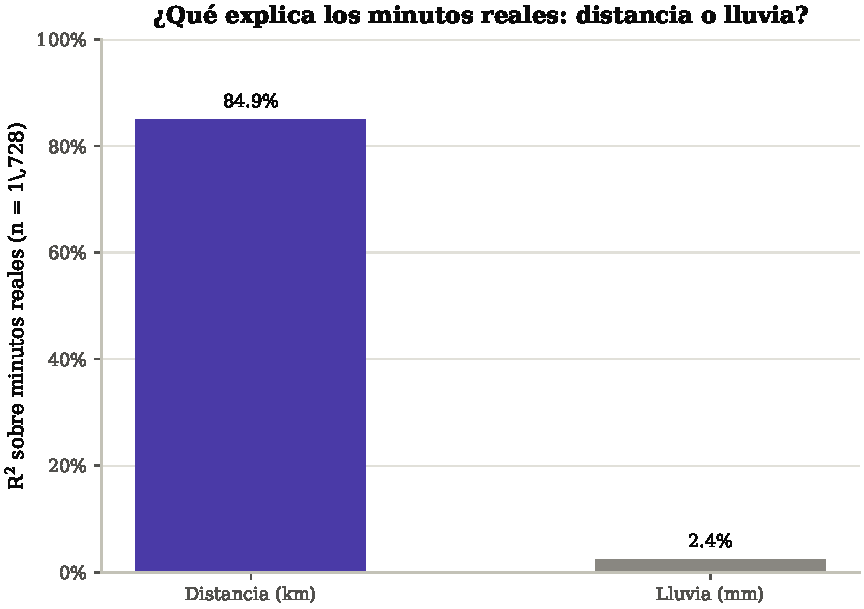
\includegraphics[width=0.85\linewidth]{caso2_q1_r2.pdf}
\caption{$R^2$ de dos asociaciones sobre \texttt{minutos\_reales}: distancia (84.9\,\%, fuerte) frente a lluvia (2.4\,\%, débil). La comparación desmonta la etiqueta de ``prueba científica'' del gráfico original.}
\label{fig:c2-q1}
\end{figure}

\paragraph{Decisión.} Retirar la etiqueta ``prueba científica''; reportar $\mathrm{corr}(\text{lluvia}, \text{minutos\_reales})$ junto a $\mathrm{corr}(\text{distancia}, \text{minutos\_reales})$ en el mismo texto para dar contexto de magnitud relativa; usar lenguaje de asociación (``se observa una diferencia promedio de $X$ minutos\ldots'') en vez de causal.

\paragraph{Límite / trade-off (matiz honesto).} Aunque el $R^2$ de la lluvia sobre los minutos crudos es bajo, al mirar el incumplimiento binario de SLA (\lstinline|tardanza_flag|) la brecha es mayor: 32.7\,\% = 411/1\,256 envíos sin lluvia frente a 76.5\,\% = 361/472 envíos con lluvia, y esa brecha persiste dentro de cada tercil de distancia (aproximadamente 32--34\,\% sin lluvia frente a 72--81\,\% con lluvia en distancia corta, media y larga; desarrollo completo en la Pregunta~4). Es decir: la lluvia no es irrelevante para el incumplimiento de SLA, pero sigue sin poder llamarse ``causa'' sin controlar transportista, vehículo y factores no medidos (tráfico, hora del día, prioridad de envío).

\subsection{Pregunta 2 --- La pregunta dicta el gráfico}\label{ssec:c2-q2}

\paragraph{Vista 1 --- comparar mediana y dispersión de \texttt{minutos\_reales} entre transportistas, dentro de cada macrozona.}

\paragraph{Concepto técnico.} La tarea analítica declarada es \emph{comparar distribuciones} --- no un solo promedio puntual --- entre 3 grupos (transportista) anidados en 3 facetas (macrozona). La marca correspondiente es el \textbf{boxplot} (posición = mediana y cuartiles; longitud de la caja = rango intercuartílico), el estándar para mostrar tendencia central y dispersión de forma simultánea.

\paragraph{Evidencia.} Las medianas por transportista $\times$ macrozona van de 166.1\,min (Apu Express--Sierra, $n=280$) a 197.8\,min (Costa Norte--Sierra, $n=250$); el rango intercuartílico (dispersión) va de \textasciitilde 97\,min (Apu Express--Selva) a \textasciitilde 140\,min (Costa Norte--Sierra); el tamaño de cada celda varía de $n=121$ (Río Rápido--Selva) a $n=280$ (Apu Express--Sierra). Ver Figura~\ref{fig:c2-q2-box}.

\begin{figure}[H]
\centering
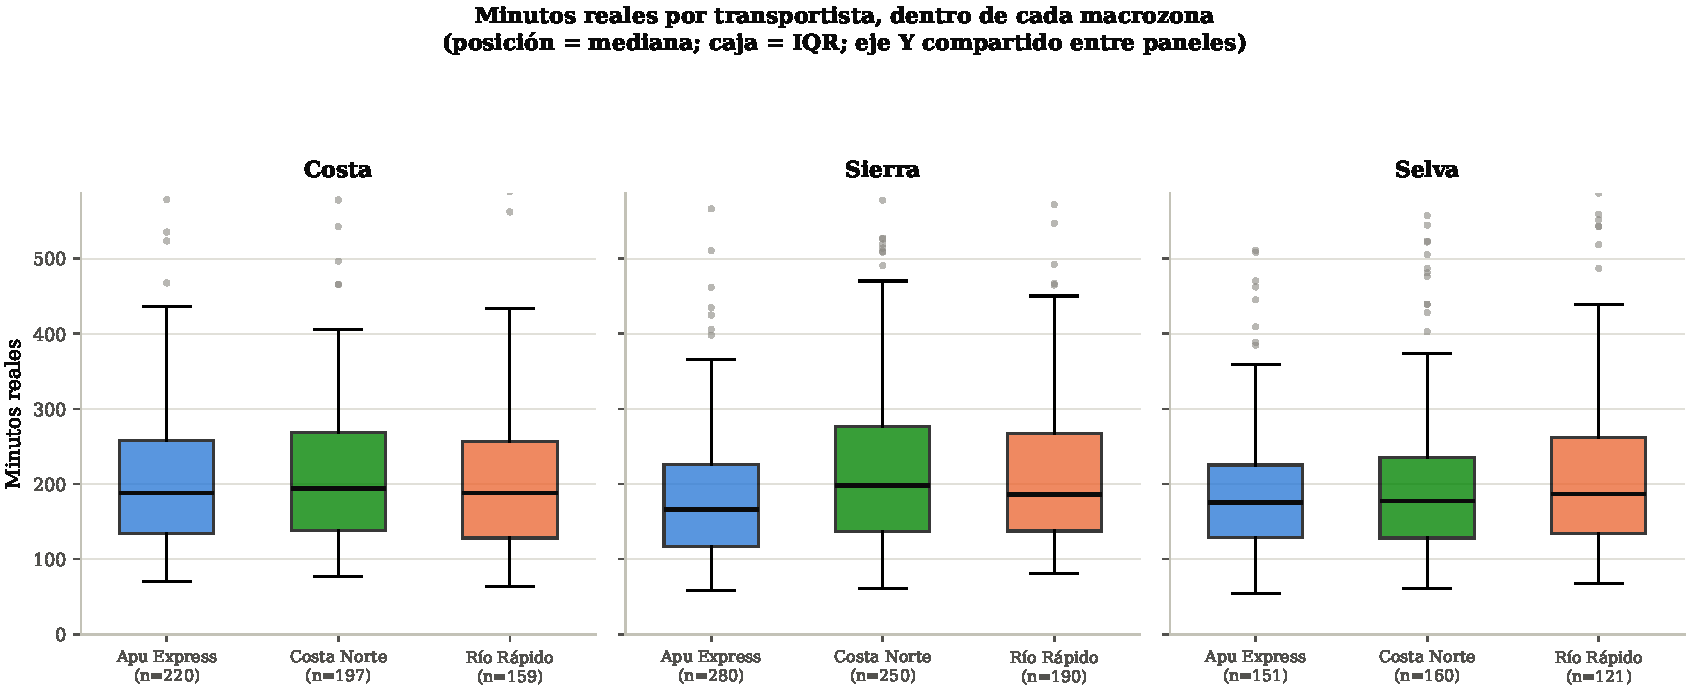
\includegraphics[width=\linewidth]{caso2_q2_box.pdf}
\caption{Distribución de \texttt{minutos\_reales} por transportista, faceteada por macrozona, con eje Y compartido en los tres paneles. La posición de la mediana y la altura de la caja son el canal más preciso para comparar tendencia central y dispersión.}
\label{fig:c2-q2-box}
\end{figure}

\paragraph{Decisión.} Eje Y = \lstinline|minutos_reales| (posición, el canal más preciso de la jerarquía posición $>$ longitud $>$ ángulo $>$ área $>$ color); eje X = transportista; facet por macrozona con eje Y compartido (mismo rango en los tres paneles) para permitir comparación directa entre paneles; color de la caja = transportista, redundante con la posición en X (no es el único canal de identificación); mediana marcada con línea gruesa; outliers mostrados como puntos, no eliminados.

\paragraph{Límite / trade-off.} El boxplot esconde la forma exacta de la distribución (por ejemplo, bimodalidad) y minimiza la lectura de $n$ si no se anota explícitamente; aquí $n$ varía de 121 a 280 por celda, anotado en las etiquetas del eje X para no sobre-interpretar cajas con pocos datos.

\paragraph{Vista 2 --- relación entre \texttt{distancia\_km} y \texttt{minutos\_reales}.}

\paragraph{Concepto técnico.} La tarea analítica declarada es \emph{evaluar la fuerza y la forma de una relación entre dos variables cuantitativas continuas}. La marca correspondiente es el \textbf{scatter plot} (posición X-Y, el canal más preciso posible para dos cuantitativas), muy superior a intentar comprimir esta relación en líneas o doble eje como en el gráfico original.

\paragraph{Evidencia.} $\mathrm{corr}=0.922$, $R^2=84.9$\,\%; recta OLS con $p\approx 0$ y $n=1\,728$:
\[
\widehat{\text{minutos\_reales}} = 1.43 \cdot \text{distancia\_km} + 60.1 .
\]
El tratamiento de valores atípicos con la regla $1.5\times$IQR marca 62 outliers en \lstinline|minutos_reales| ($>444.1$\,min, 3.6\,\%) y 49 outliers en \lstinline|distancia_km| ($>260.8$\,km, 2.8\,\%). Ver Figura~\ref{fig:c2-q2-scatter}.

\begin{figure}[H]
\centering
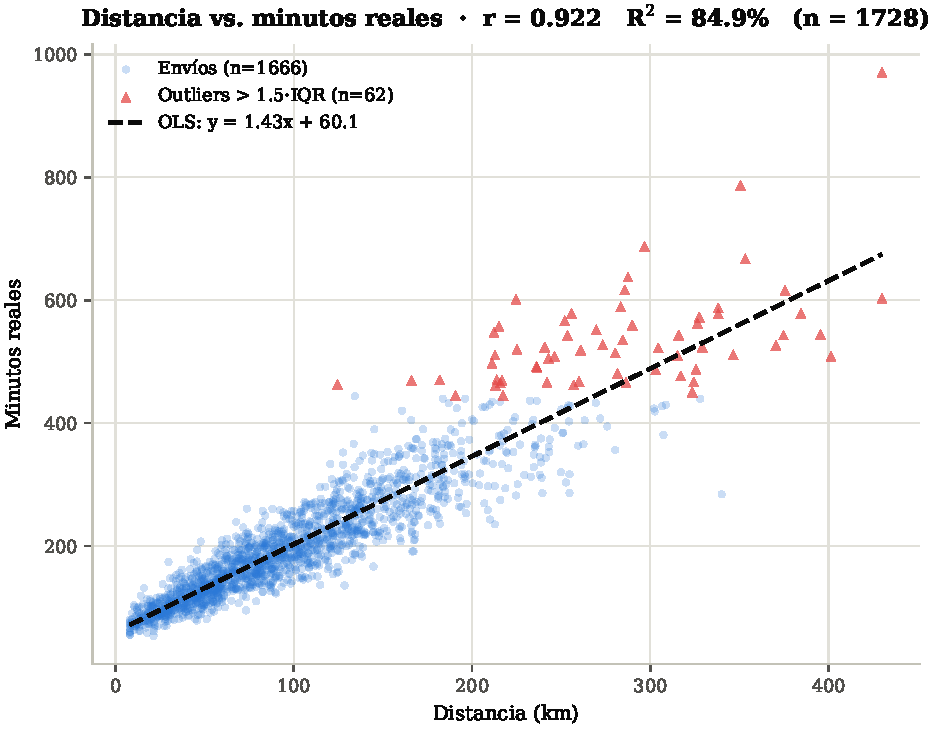
\includegraphics[width=0.85\linewidth]{caso2_q2_scatter.pdf}
\caption{Distancia frente a minutos reales (n = 1\,728), con recta OLS y outliers ($>1.5\cdot$IQR) resaltados en vez de eliminados.}
\label{fig:c2-q2-scatter}
\end{figure}

\paragraph{Decisión.} Transparencia (alpha = 0.25) para mitigar el sobre-trazado (\emph{overplotting}) de 1\,728 puntos; línea de tendencia OLS anotada con su ecuación y $R^2$; los outliers no se eliminan --- se resaltan con marcador y color distintos porque representan casos reales de negocio (por ejemplo, camiones a distancias largas en Selva) que la gerencia necesita ver, no ocultar.

\paragraph{Límite / trade-off.} La recta OLS asume una relación lineal y homocedástica; a distancias muy largas la dispersión podría crecer (heterocedasticidad), por lo que antes de usar esta recta para pronóstico habría que revisar residuales por tramo de distancia. Además, eliminar outliers ``para limpiar el gráfico'' sin justificación operativa ocultaría exactamente los envíos que más le cuestan a la operación.

\paragraph{Elección de KPI principal: tasa de tardanza vs.\ SLA, con P90 como \emph{guardrail}.}

\paragraph{Concepto técnico.} Un KPI operacional debe ser accionable frente a una meta, no solo descriptivo de una distribución.

\paragraph{Evidencia.} Periodo: 18 semanas, \lstinline|semana_inicio| del 2026-03-02 al 2026-06-29. Tasa de tardanza agregada = 772/1\,728 = 44.68\,\% frente a una meta de 20\,\% (más del doble). El P90 por transportista (Apu Express 312.8\,min, Costa Norte 354.2\,min, Río Rápido 349.9\,min) muestra la cola; la media (193.8 / 212.8 / 212.3\,min) está sesgada por outliers y por la mezcla de distancias; la mediana (175.3 / 187.4 / 187.3\,min) es robusta pero esconde justamente esa cola.

\paragraph{Decisión.} Se recomienda la \textbf{tasa de tardanza vs.\ SLA} ($\text{SUM}(\text{tardanza\_flag})/\text{COUNT}(\text{envio\_id})$) como KPI decisor primario --- es binario, está directamente ligado a la meta operativa del 20\,\% y admite una línea de referencia clara (Pregunta~4) --- usando \textbf{P90} como \emph{guardrail} de cola, con un umbral propuesto de meta P90 $\le 300$\,min (los tres transportistas ya lo superan: 312.8--354.2\,min), para detectar si el 10\,\% peor de envíos se dispara aunque la mediana luzca aceptable.

\begin{lstlisting}[style=cod]
Mediana por celda (Tableau):     { FIXED [Macrozona],[Transportista] : MEDIAN([Minutos Reales]) }
Mediana por celda (pandas):      df.groupby(['macrozona','transportista'])['minutos_reales'].median()

P90 por transportista (Tableau): { FIXED [Transportista] : PERCENTILE([Minutos Reales], 0.9) }
P90 por transportista (pandas):  df.groupby('transportista')['minutos_reales'].quantile(0.9)

Tasa de tardanza (Tableau):      SUM([Tardanza_flag]) / COUNT([Envio_id])   -- con [Transportista] en Filas
Tasa de tardanza (pandas):       df.groupby('transportista')['tardanza_flag'].agg(['sum','count'])
\end{lstlisting}

\paragraph{Límite / trade-off.} La media es sensible a outliers y a cambios en el mix de rutas (una semana con más envíos largos la mueve sin que cambie el desempeño real por ruta); la mediana esconde la cola (el P90 puede duplicarse sin que la mediana se mueva); la tasa de tardanza sola no dice \emph{cuánto} tarde llega un envío, por lo que se complementa con el P90; ninguno de los cuatro estadísticos controla por transportista o macrozona por sí solo --- deben reportarse siempre segmentados, no solo en agregado.

\subsection{Pregunta 3 --- Doce series sin espagueti}\label{ssec:c2-q3}

Tarea analítica declarada: seguir la evolución semanal de la tasa de tardanza por sede para detectar cuáles sedes están sistemáticamente por encima de la meta, sin perder la capacidad de comparar magnitudes entre sedes.

\paragraph{Concepto técnico.} Con 12 series de solo 18 puntos cada una y ruido alto (ver evidencia), superponerlas en un único plano es un antipatrón de selección de gráfico. La solución es \textbf{pequeños múltiplos} (facet por sede) combinados con \textbf{foco + contexto} (la sede de cada panel resaltada en color, las otras 11 dibujadas en gris de fondo como referencia): así se preserva tanto la comparación ``dentro de panel vs.\ meta'' como la comparación ``entre sedes'' sin espagueti ni leyenda de 12 colores.

\paragraph{Evidencia.} 12 sedes $\times$ 18 semanas = 216 celdas sede-semana, cada una con exactamente 8 envíos (mínimo = mediana = máximo = 8), por lo que la tasa semanal de una sede solo puede tomar valores en incrementos de 12.5 puntos porcentuales (0\,\%, 12.5\,\%, \ldots, 87.5\,\%): un solo envío que cruza el umbral mueve la tasa 12.5\,pp de golpe. Con 8 envíos por sede-semana $\times$ 18 semanas = 144 envíos por sede, la sede con peor tasa agregada es SED-01 (Lima, Costa) con 61.1\,\% = 88/144; la mejor es SED-04 (Chiclayo, Costa) con 28.5\,\% = 41/144 (Figura~\ref{fig:c2-q3}).

\begin{figure}[H]
\centering
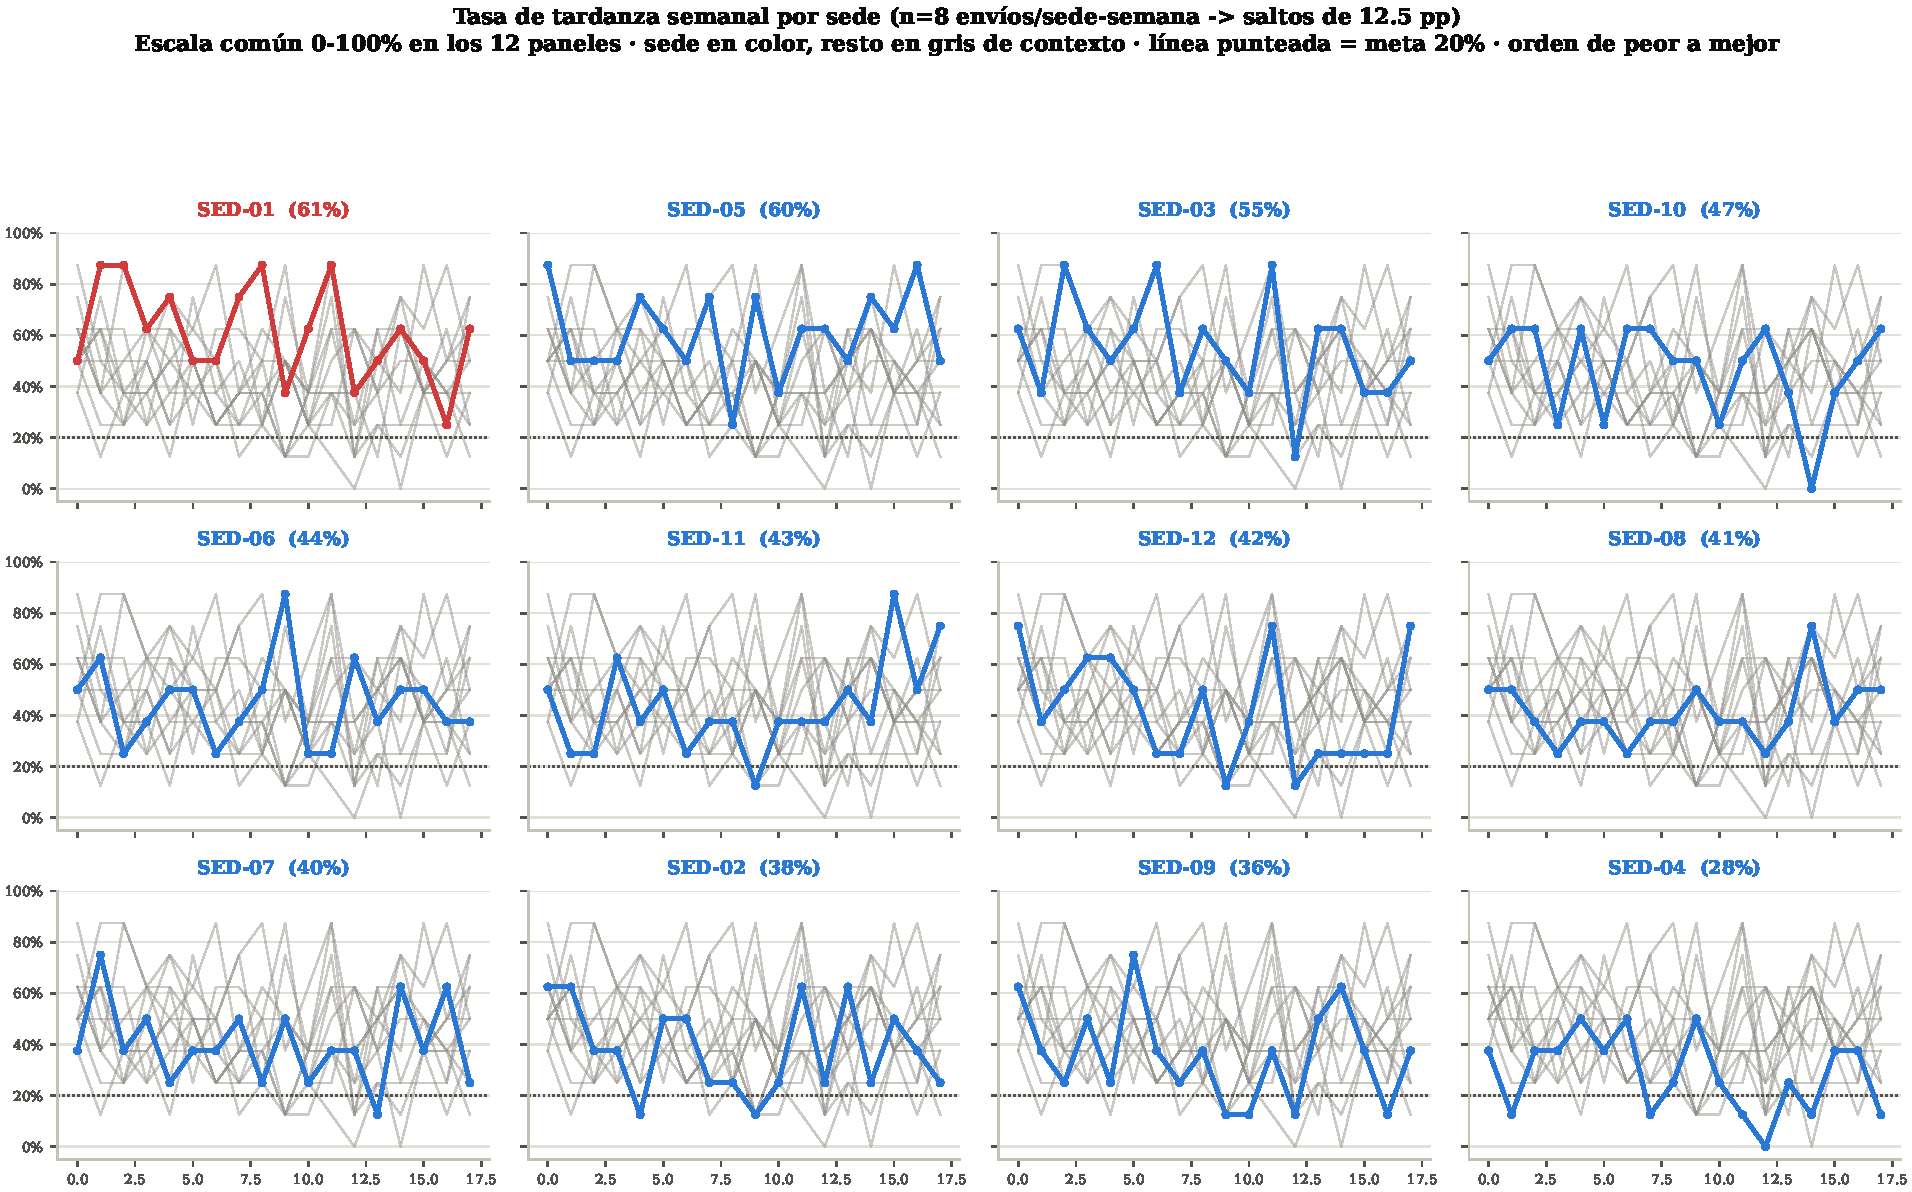
\includegraphics[width=\linewidth]{caso2_q3_multiplos.pdf}
\caption{Tasa de tardanza semanal por sede, 12 pequeños múltiplos con escala común 0--100\,\% y línea de meta al 20\,\%. Cada panel resalta su propia sede (SED-01, la peor, en rojo) sobre las otras 11 en gris de contexto; orden de peor a mejor por tasa agregada.}
\label{fig:c2-q3}
\end{figure}

\paragraph{Decisión.} Escala compartida de 0 a 100\,\% en los 12 paneles (nunca autoescalada), condición no negociable para que la altura de cada línea sea comparable entre paneles. Etiquetado directo: el nombre de la sede y su tasa agregada se imprimen como título del panel (texto), sin leyenda de color para 12 series. El significado no depende del matiz sino de la posición de la línea coloreada respecto a la línea de referencia (meta 20\,\%, punteada) y de la etiqueta de texto directa; en escala de grises, la línea focal (más gruesa, con marcadores) sigue siendo distinguible del fondo gris tenue por grosor y opacidad, no solo por color. La línea de referencia de meta (20\,\%) se repite en cada panel para un juicio inmediato de ``por encima / por debajo''. El \emph{table calc} que ordena los paneles se declara explícitamente: $\mathrm{RANK}(\mathrm{SUM}(\text{tardanza\_flag})/\mathrm{COUNT}(\text{envio\_id}))$ con \textbf{partición = ninguna} (toda la tabla es una sola partición) y \textbf{addressing = sede\_id} (recorre las 12 sedes, sin reinicio).

\paragraph{Límite / trade-off.} Si cada panel usara su propio eje Y ajustado al rango local de esa sede, una sede de bajo desempeño real (por ejemplo, SED-04, 28.5\,\% agregado, con variación semana a semana pequeña en términos absolutos) podría verse tan ``dramática'' en su panel como SED-01 (61.1\,\%), porque el eje se estira para llenar el espacio del panel: es una ilusión creada por el diseño (autoescalado), no por la magnitud real de los datos --- motivo exacto por el que se fija la escala compartida 0--100\,\%. Además, con 8 envíos por semana, un solo pico aislado no debe leerse como tendencia: se recomienda no interpretar un salto de 12.5\,pp sin mirar al menos 3--4 semanas consecutivas o el agregado del panel.

\subsection{Pregunta 4 --- Declarar no es inferir}\label{ssec:c2-q4}

\paragraph{KPI decisor: tasa de tardanza agregada vs.\ meta.}

\paragraph{Concepto técnico.} Una línea de referencia de meta convierte una tasa descriptiva en un juicio operativo binario (¿cruza o no cruza la meta?); no es un promedio ilustrativo, es un umbral de decisión.

\paragraph{Evidencia.} $\text{num}$ (envíos con \lstinline|tardanza_flag|=1) = 772; $\text{den}$ (envíos totales) = 1\,728; tasa de tardanza agregada = 772/1\,728 = 44.68\,\%. Periodo: 18 semanas, \lstinline|semana_inicio| del 2026-03-02 al 2026-06-29. Segmento: agregado, todas las sedes y transportistas. Meta operativa declarada: 20\,\%. El KPI está 24.68 puntos porcentuales por encima de la meta (2.23$\times$ la meta). Como verificación de robustez del campo fuente: la regla operativa \lstinline|tardanza_flag| = 1 si \lstinline|minutos_reales| $\ge 1.12\times$\lstinline|minutos_objetivo| reproduce el campo \lstinline|tardanza_flag| en 1\,727 de 1\,728 filas (99.94\,\%); el único caso discrepante (ratio = 1.119962, a 0.038\,pp del corte) es redondeo de piso, no una regla distinta, por lo que \lstinline|tardanza_flag| se trata como campo autoritativo para todo cálculo de tasas.

\paragraph{Decisión.} Dibujar una línea de referencia horizontal en 20\,\% sobre la serie o barra de tasa de tardanza (Figura~\ref{fig:c2-q1} sirve de referencia de estilo; ver también Figura~\ref{fig:c2-q3} para la meta por sede) y reportar siempre $\text{num}/\text{den}$ junto al porcentaje, nunca el porcentaje solo. Fórmula Tableau: \texttt{SUM([Tardanza\_flag]) / COUNT([Envio\_id])}, con línea de referencia constante en 0.20 (campo calculado \texttt{Meta = 0.20} o parámetro). Pandas: \texttt{df['tardanza\_flag'].sum() / len(df)}.

\paragraph{Límite / trade-off.} La tasa agregada mezcla transportistas muy distintos (Apu Express 32.4\,\% = 211/651 frente a Río Rápido 57.2\,\% = 269/470, con Costa Norte en 48.1\,\%) y sedes muy distintas (SED-04 28.5\,\% = 41/144 frente a SED-01 61.1\,\% = 88/144): cruzar la meta en agregado no dice \emph{dónde} actuar; siempre debe acompañarse de la vista segmentada (Preguntas~2 y~3) antes de tomar una decisión de asignación.

\paragraph{Trend line lluvia--demora: una pregunta distinta, no causal.}

\paragraph{Concepto técnico.} Una recta de tendencia (OLS) entre \lstinline|lluvia_mm| y \lstinline|minutos_reales| responde a la pregunta ``¿cuál es la mejor recta lineal que resume cómo covarían estas dos variables en los datos observados?'' --- una pregunta descriptiva y asociativa (¿cuánto se mueve $Y$ en promedio por unidad de $X$, en esta muestra?), \textbf{no} la pregunta causal ``¿si yo pudiera cambiar la lluvia manteniendo todo lo demás fijo, cambiaría el tiempo de entrega?''. Esta segunda pregunta requiere un diseño que aísle la lluvia de sus covariables (experimento o cuasi-experimento), algo que un CSV observacional de un solo periodo no ofrece \citep{anscombe1973graphs}.

\paragraph{Evidencia.} OLS lluvia $\to$ minutos reales ($r=0.156$, $R^2=2.4$\,\%, $p=6.8\times 10^{-11}$):
\[
\widehat{\text{minutos\_reales}} = 2.01 \cdot \text{lluvia\_mm} + 198.2 ,
\]
significativo pero de efecto pequeño sobre los minutos crudos. Sin embargo, sobre \lstinline|tardanza_flag| la asociación sin controlar es mayor: 32.7\,\% = 411/1\,256 (sin lluvia) frente a 76.5\,\% = 361/472 (con lluvia), y esa brecha de 38 a 48 puntos porcentuales persiste dentro de cada tercil de distancia --- corta (37.8\,pp), media (45.9\,pp) y larga (47.9\,pp). Transportista y vehículo están balanceados entre los grupos con y sin lluvia (proporciones casi idénticas por transportista y por vehículo entre \lstinline|lluvia_flag|=0 y =1), por lo que no son confusores fuertes de la exposición; la macrozona sí varía en incidencia de lluvia (Selva 41.7\,\% = 180/432 frente a Costa 16.5\,\% = 95/576) pero su tasa de tardanza propia es casi plana (Costa 45.7\,\%, Sierra 44.4\,\%, Selva 43.8\,\%), por lo que tampoco explica la brecha por sí sola.

\paragraph{Decisión.} Antes de confiar en la trend line se revisarían dos supuestos: primero, \textbf{linealidad} --- ¿el efecto de la lluvia es realmente lineal en mm, o hay un umbral (``llueve o no llueve'' importa más que los mm exactos)? El salto grande en \lstinline|tardanza_flag| frente al $R^2$ bajo en minutos crudos sugiere un efecto de umbral sobre el \emph{ratio} minutos\_reales/objetivo ($\mathrm{corr}(\text{lluvia\_mm}, \text{ratio}) = 0.489$, muy superior a $\mathrm{corr}(\text{lluvia\_mm}, \text{minutos\_reales}) = 0.156$), no una recta continua. Segundo, \textbf{confusores}: distancia ($r=0.922$ con el resultado, pero $r=0.001$ con lluvia, por lo que no es confusor clásico de la relación lluvia-minutos, aunque sí domina la varianza total); transportista y vehículo (balanceados, verificado arriba); macrozona (asociada a la exposición, pero con tasa de tardanza propia casi plana); y factores no medidos (tráfico, hora del día, prioridad de envío, día de semana) que podrían covariar con la lluvia y explicar parte de la brecha.

\paragraph{Límite / trade-off.} Ni una pendiente ni un buen $R^2$ demuestran causalidad: los datos son observacionales --- nadie asignó aleatoriamente qué envíos ``reciben'' lluvia --- y un $R^2$ alto solo certifica buen ajuste dentro de la muestra, no aislamiento de la causa. Aquí, además, el $R^2$ de la lluvia sobre los minutos crudos es bajo (2.4\,\%) precisamente porque la distancia domina la varianza (84.9\,\%); mezclar ambas señales en un gráfico de doble eje, como hacía el original, es lo que producía la ilusión de ``prueba científica''.

\bitacora{
``La lluvia parece causar toda la tardanza; el gráfico de 12 líneas lo prueba.''
}{
Tasa de tardanza vs.\ SLA --- Tableau \texttt{SUM([Tardanza\_flag])/COUNT([Envio\_id])}, pandas \texttt{df['tardanza\_flag'].sum()/len(df)} --- periodo 2026-03-02 a 2026-06-29 (18 semanas) --- segmento agregado y por transportista/sede --- meta 20\,\%.
}{
Al descomponer por distancia y transportista, la distancia explica el 84.9\,\% de la varianza de \texttt{minutos\_reales} ($r=0.922$) frente al 2.4\,\% de la lluvia ($r=0.156$); Río Rápido (57.2\,\% = 269/470 tardíos) casi duplica a Apu Express (32.4\,\% = 211/651): el problema es mayormente operativo (ruteo/transportista), no meteorológico, aunque la lluvia sigue asociada al incumplimiento de SLA dentro de cada tercil de distancia.
}{
``Distancia y transportista se asocian con la tardanza; la lluvia es secundaria pero no nula.''
}{
La decisión que cambia es priorizar la renegociación de rutas y SLA con Río Rápido y Costa Norte, y revisar la asignación en distancias largas, en vez de invertir primero en ``gestión de lluvia''. El dato que refutaría esta lectura revisada sería una regresión múltiple (\texttt{lluvia\_flag} + \texttt{distancia\_km} + transportista + vehículo + macrozona + semana) donde el coeficiente de \texttt{lluvia\_flag} deje de ser significativo tras controlar todo lo demás, o, mejor aún, un experimento o cuasi-experimento que compare la misma ruta, transportista y vehículo en semanas con y sin lluvia y muestre que la tardanza no cambia; si en cambio el coeficiente de lluvia se mantiene significativo y de magnitud relevante tras esos controles, habría que reincorporar la lluvia como factor operativo real --- no como ``prueba científica'' única, sino como covariable relevante junto a distancia y transportista.
}

\section{Caso 3 --- Julio duró doce días y el titular duró para siempre}
\label{sec:caso3}

El dataset de este caso (\texttt{data/caso3\_asistencia\_mensual\_chasquifest.csv}) tiene granularidad de una fila por mes $\times$ sede: 372 filas (31 meses, ene-2024 a jul-2026, por 12 sedes). Los campos relevantes son \texttt{mes}, \texttt{anio}, \texttt{numero\_mes}, \texttt{sede\_id}, el par \texttt{dias\_observados}/\texttt{dias\_del\_mes} (completitud del periodo), \texttt{cobertura\_periodo\_pct}, \texttt{asistentes} (volumen \emph{observado}, no proyectado), \texttt{meta\_asistentes} (ya ajustada a los días observados) y \texttt{evento\_contexto} (marca el quiebre logístico ficticio).

El disparador del caso es editorial: se compara julio-2026 --- con corte a 12 días --- contra julio-2025 \textbf{completo} (31 días) y se anuncia una caída del 57\%. La verificación directa del CSV confirma los totales, pero expone el problema de fondo: \textbf{no son periodos homólogos}. Julio-2025 tiene \texttt{dias\_observados}=31/31 (cobertura 100\%) y un total de 281\,044 asistentes; julio-2026 tiene \texttt{dias\_observados}=12/31 (cobertura 38.71\%) y un total de 121\,281 asistentes. Comparar un mes cerrado contra uno truncado a poco menos de dos quintas partes de sus días mezcla desempeño con exposición temporal --- exactamente el error que las cuatro preguntas siguientes diagnostican y corrigen.

\subsection{Pregunta 1 --- Componentes de la serie: tendencia, estacionalidad, quiebre y cobertura}
\label{ssec:c3-q1}

\paragraph{Concepto técnico.}
Toda serie mensual observada se descompone en tendencia (nivel de largo plazo), estacionalidad (patrón que se repite cada año en los mismos meses), ruido (variación mes a mes no explicada por lo anterior) y, cuando existe, un quiebre estructural (choque puntual y localizado que no es ni tendencia ni estacionalidad):
\[
\text{asistentes}_t \;=\; \text{tendencia}_t + \text{estacionalidad}_t + \text{quiebre}_t + \text{ruido}_t .
\]
Julio-2026 exige un quinto componente, ortogonal a los anteriores: la \textbf{cobertura o completitud del periodo}. Cuando \texttt{dias\_observados} $<$ \texttt{dias\_del\_mes}, el valor no es un punto cerrado de la serie sino una medición parcial, ligada al total pleno por
\[
\text{asistentes}_{\text{observado},\,t} \;\approx\; \text{asistentes}_{\text{pleno},\,t}\times\frac{\text{dias\_observados}_t}{\text{dias\_del\_mes}_t}\quad(\text{bajo el supuesto de afluencia diaria uniforme}).
\]

\paragraph{Evidencia.}
\textbf{Tendencia (leve alza):} el total anual de \texttt{asistentes} pasa de 2\,471\,862 en 2024 a 2\,703\,721 en 2025 (+9.38\%); los doce meses de 2025 superan a su homólogo 2024 sin excepción, entre +3.60\% (abril) y +15.58\% (febrero). Incluso marzo--mayo de 2025 --- los meses del quiebre --- crecen frente a 2024 (mar +11.16\%, abr +3.60\%, may +6.24\%), porque el quiebre solo golpea 2 de 12 sedes y no rompe la tendencia agregada.
\textbf{Estacionalidad (picos jul/dic):} en 2025, julio = 281\,044 y diciembre = 321\,462, frente a una base de meses no-pico que oscila entre 183\,751 (feb) y 226\,442 (nov), con media $\approx$210\,122; el mismo patrón se repite en 2024 (jul = 250\,847, dic = 292\,448). Es estructural y recurrente cada año.
\textbf{Ruido:} oscilación mes a mes sin patrón --- p.\,ej., 2025: ene 206\,593 $\rightarrow$ feb 183\,751 (-11.06\%) $\rightarrow$ mar 203\,347 (+10.66\%).
\textbf{Quiebre (Loreto/Ucayali, mar--may 2025):} SED-11 (Iquitos) y SED-12 (Pucallpa) registran \texttt{evento\_contexto}=\enquote{Interrupción logística ficticia} en exactamente 6 de 372 filas. Iquitos cae a 8\,518 / 8\,485 / 7\,459 asistentes (índice $\approx$63.5 / 63.3 / 55.6 sobre su propio enero-2025 = 13\,411); Pucallpa cae a 7\,429 / 7\,109 / 7\,147 (índice $\approx$66.1 / 63.2 / 63.6 sobre enero-2025 = 11\,242). Ambas sedes se recuperan en junio-2025 (Iquitos 13\,665 = índice 101.9; Pucallpa 11\,520 = índice 102.5): es un evento localizado y temporal en forma de \enquote{V}, no una tendencia estructural nueva. El resto de sedes y meses (366/372 filas) marca \enquote{Sin quiebre registrado}, y en 2026 ambas sedes vuelven a esa etiqueta en las 14 filas correspondientes.
\textbf{Julio 2026:} \texttt{dias\_observados}=12, \texttt{dias\_del\_mes}=31, \texttt{cobertura\_periodo\_pct}=38.71\%, total = 121\,281.

\paragraph{Decisión.}
Julio-2026 no se etiqueta automáticamente ni como \enquote{caída} ni como \enquote{outlier}. Para sostener \enquote{caída} se necesita una comparación entre periodos homólogos (misma cobertura); comparar el total de 12 días contra el total de 31 días del año anterior --- un \texttt{LOOKUP(..., -12)} ingenuo --- no lo es. Para sostener \enquote{outlier} hay que descartar primero que la anomalía se explique por cobertura: aquí se explica enteramente por ella. Un chequeo sobre las 31 combinaciones año$\times$mes del dataset confirma que julio-2026 (38.71\%) es el \emph{único} periodo con \texttt{cobertura\_periodo\_pct} $<$ 100\% en las 372 filas; todos los demás meses de la serie cierran con cobertura 100\%. El diagnóstico correcto es \textbf{periodo truncado / observación incompleta}, no un evento del negocio. Titular inicial (el que produce el gráfico ingenuo): \enquote{Julio se desploma 57\%: la asistencia colapsa en ChasquiFest.} Titular revisado, tras auditar \texttt{cobertura\_periodo\_pct}: \enquote{Julio-2026 solo tiene 12 de 31 días registrados (38.71\% de cobertura); al ritmo diario observado, la asistencia va +11.5\% por encima de julio-2025} (ver Pregunta~\ref{ssec:c3-q3}).

\paragraph{Límite / trade-off.}
Clasificar automáticamente por umbral (p.\,ej., \enquote{toda caída $>$50\% es alerta roja}) es peligroso si el \emph{pipeline} de reporting no verifica \texttt{cobertura\_periodo\_pct} antes de calcular variaciones: el mismo dato produce una alerta falsa de crisis o una lectura correcta de crecimiento, según se audite o no la completitud primero.

La Figura~\ref{fig:c3-q1} muestra la serie completa: tendencia leve al alza, picos estacionales de julio y diciembre, la banda del quiebre Loreto/Ucayali (mar--may 2025) y julio-2026 resaltado con su cobertura de 38.71\%.

\begin{figure}[H]
\centering
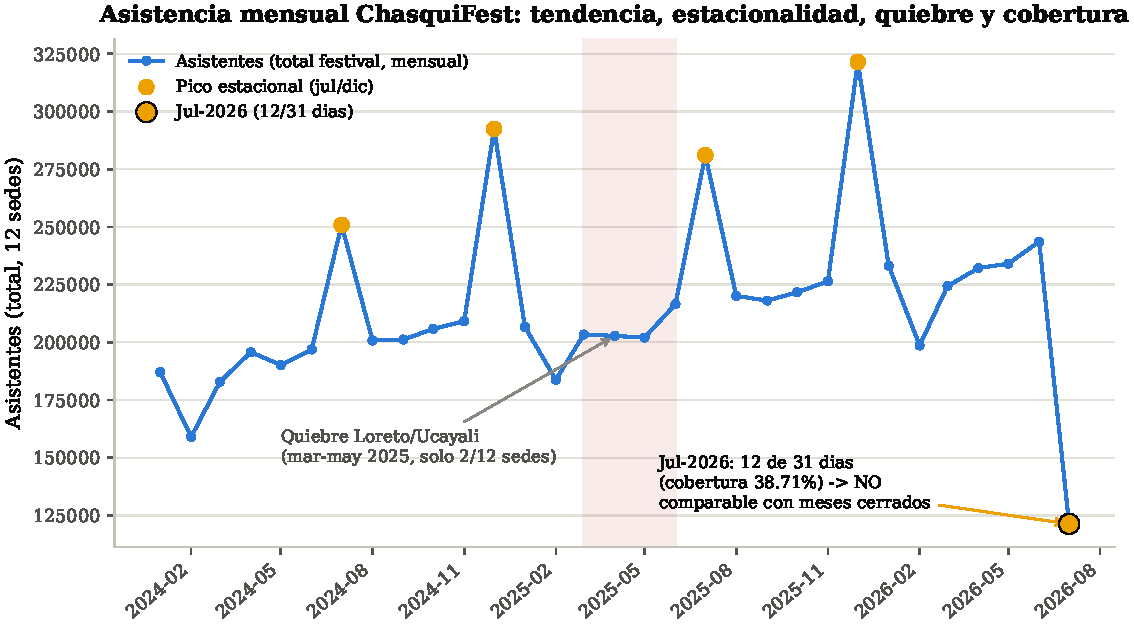
\includegraphics[width=0.85\linewidth]{caso3_q1_serie.pdf}
\caption{Serie mensual de asistentes (todas las sedes, ene-2024 a jul-2026): tendencia leve al alza, picos estacionales de julio y diciembre, banda del quiebre Loreto/Ucayali (mar--may 2025) y julio-2026 truncado a 12 de 31 días (cobertura 38.71\%).}
\label{fig:c3-q1}
\end{figure}

\subsection{Pregunta 2 --- Ventana, acumulado y dirección}
\label{ssec:c3-q2}

\paragraph{Concepto técnico.}
Una media móvil (\emph{window function} \texttt{WINDOW\_AVG}) suaviza estacionalidad y ruido para leer la dirección reciente del nivel de la serie. Un acumulado (\texttt{RUNNING\_SUM}) mide progreso hacia una meta dentro de una ventana temporal --- típicamente el año --- y, por diseño, es monótono no decreciente si la métrica es siempre $\geq 0$. Responden preguntas distintas (\enquote{tasa/nivel} frente a \enquote{stock acumulado}) y no deben graficarse en el mismo eje sin declarar esa diferencia de semántica \citep{few2009now}.

\paragraph{Evidencia.}
\begin{lstlisting}[style=cod]
// (a) Media movil de 3 meses (total festival)
WINDOW_AVG(SUM([asistentes]), -2, 0)
// (b) Acumulado que reinicia cada anio (YTD)
RUNNING_SUM(SUM([asistentes]))
\end{lstlisting}
\textbf{(a)} Addressing: \texttt{Along Mes} (table-down si \texttt{Mes} está en filas). Partición: sin partición por sede, porque este cálculo usa el total festival ya agregado por mes (con partición por \texttt{Sede} se obtendría la media móvil de cada sede por separado). Orden: \texttt{Mes} ascendente --- obligatorio para que \texttt{-2,0} tome \enquote{los 2 meses previos + el actual}. Símil pandas: \texttt{serie.groupby('mes')['asistentes'].sum().sort\_index().rolling(3).mean()}.
\textbf{(b)} Addressing: \texttt{Along Mes}. Partición/reinicio: \texttt{compute using Mes, restarting every Año} --- el acumulado vuelve a 0 en enero de cada año. Orden: \texttt{Mes} ascendente dentro de cada año. Símil pandas: \texttt{serie.groupby('anio')['asistentes'].cumsum()} sobre la serie mensual ya agregada.

\paragraph{Decisión.}
Para programar el mes siguiente, el \textbf{KPI decisor} es la media móvil de 3 meses (o el YoY por ritmo diario homólogo de la Pregunta~\ref{ssec:c3-q3}): mide dirección real y reciente. El \textbf{contexto} es el acumulado YTD: sirve para verificar avance hacia la meta anual, no para decidir el mes siguiente. El acumulado es una \textbf{falsa tranquilidad} cuando se usa como KPI decisor: YTD hasta julio-2025 (mes completo) = 1\,496\,024; YTD hasta julio-2026 (mes truncado a 12 días) = 1\,487\,219 --- una diferencia de solo -0.59\%, pese a la caída bruta de -56.8\% en julio y al ritmo corregido de +11.5\% (Pregunta~\ref{ssec:c3-q3}). Un lector que solo mira el acumulado concluiría \enquote{vamos casi igual que el año pasado}, sin notar que julio está truncado: seis meses completos ya \enquote{amortiguan} cualquier mes parcial, y el acumulado nunca baja, así que jamás avisaría de un deterioro real hasta muy tarde en el año.

\paragraph{Límite / trade-off.}
La media móvil de 3 meses retrasa la detección de un quiebre 1--2 meses, y su último punto se contamina si el mes más reciente está truncado: en julio-2026 cae a 199\,654 al incluir el mes parcial, frente a 236\,608 en junio-2026 con 3 meses completos --- no es una lectura limpia del nivel reciente cuando el mes más nuevo no ha cerrado. El YTD, por construcción, nunca decrece (es la suma acumulada de una métrica $\geq0$): en el peor escenario posible seguiría subiendo mes a mes aunque el negocio se esté desplomando, solo que más lento.

La Figura~\ref{fig:c3-q2} separa ambas lecturas en dos paneles: la media móvil de 3 meses (dirección reciente, con su último punto marcado como contaminado por el mes truncado) y el acumulado YTD por año (progreso, que apenas distingue 2025 de 2026 pese a la caída bruta de julio).

\begin{figure}[H]
\centering
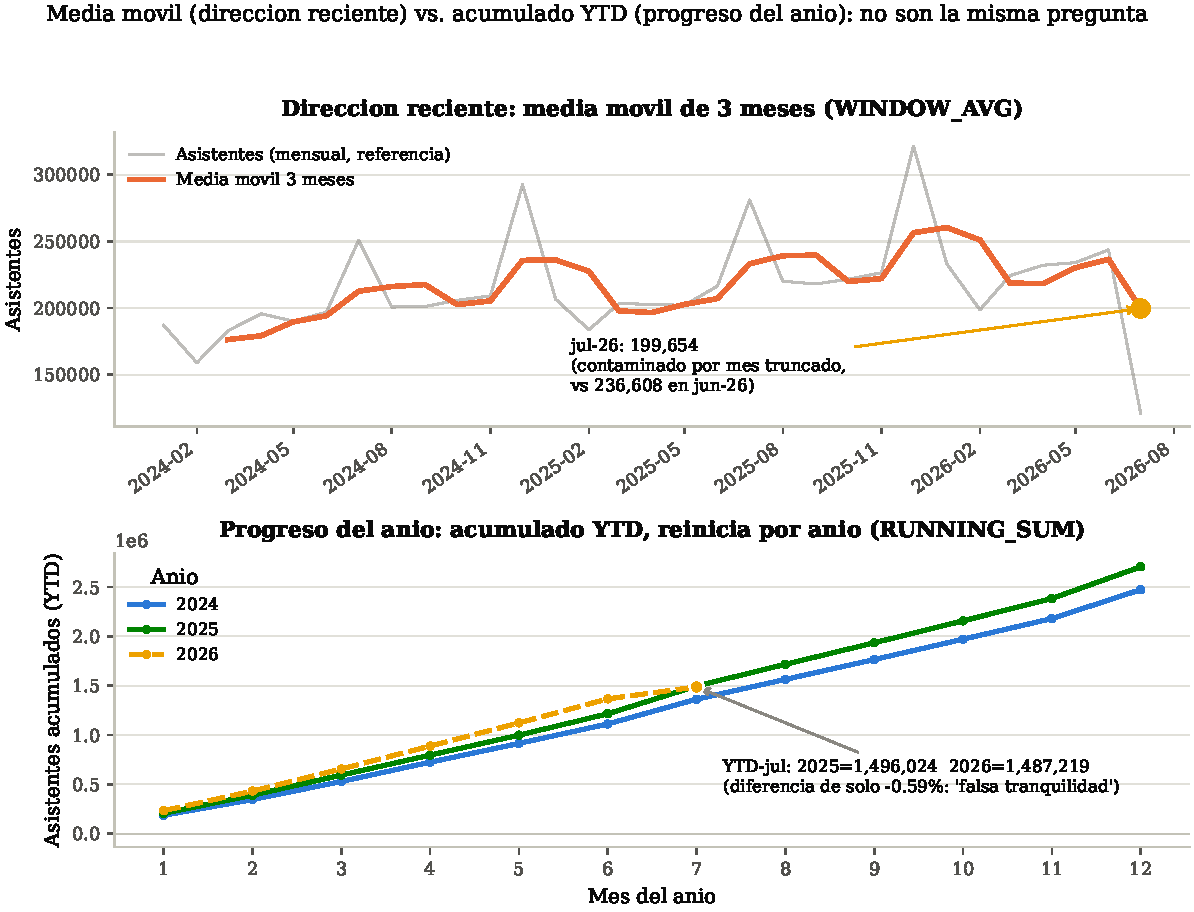
\includegraphics[width=0.85\linewidth]{caso3_q2_ma_ytd.pdf}
\caption{Panel superior: media móvil de 3 meses del total festival (dirección reciente). Panel inferior: acumulado YTD por año, reiniciado en enero. El acumulado de 2026 prácticamente iguala al de 2025 pese a la caída bruta de julio: la \enquote{falsa tranquilidad} del progreso anual.}
\label{fig:c3-q2}
\end{figure}

\subsection{Pregunta 3 --- Comparación interperiodo: el YoY válido para julio 2026}
\label{ssec:c3-q3}

\paragraph{Concepto técnico.}
Una comparación año contra año (YoY) solo es válida entre periodos homólogos: misma unidad de exposición (aquí, días observados). \texttt{LOOKUP(SUM([asistentes]), -12)} en una tabla mensual trae, para julio-2026, el valor 12 meses atrás --- julio-2025, con cobertura 100\%. Compararlo directo contra julio-2026 (cobertura 38.71\%) mezcla un mes de 31 días contra uno de 12: no son periodos homólogos, y la diferencia resultante mide sobre todo la diferencia de cobertura, no de desempeño.

\paragraph{Evidencia.}
\[
\text{caída bruta} = \frac{\text{asistentes}_{jul26} - \text{asistentes}_{jul25}}{\text{asistentes}_{jul25}} = \frac{121\,281 - 281\,044}{281\,044} = \frac{-159\,763}{281\,044} = -56.8\%
\]
compara \textbf{totales de mes} --- magnitudes con exposición distinta (31 días vs. 12 días).
\[
\text{cambio de ritmo diario} = \frac{\text{asistentes}_{jul26}/12 - \text{asistentes}_{jul25}/31}{\text{asistentes}_{jul25}/31} = \frac{10\,106.75 - 9\,065.94}{9\,065.94} = \frac{1\,040.80}{9\,065.94} = +11.48\%
\]
compara \textbf{tasas por día} --- controla la exposición. El signo se invierte (-56.8\% $\rightarrow$ +11.48\%, redondeado en el titular a -57\% y +11.5\%) sin que ningún dato del CSV cambie: lo único que cambia es el denominador --- \enquote{31 días fijos} del mes completo del año anterior frente a \enquote{días realmente observados} (12) de este año. Es la misma trampa de comparar las ventas totales de una tienda abierta 12 días del mes contra una tienda abierta los 31 días completos, sin normalizar por días de apertura.

\paragraph{Decisión.}
Tres formas de construir un YoY válido:
\textbf{(a) Días homólogos.} Ideal: comparar los primeros 12 días de julio-2025 contra los 12 días observados de julio-2026. Limitación de datos: este CSV tiene granularidad mensual $\times$ sede, no diaria --- no existe un campo para aislar \enquote{los primeros 12 días de julio-2025}. Proxy, asumiendo distribución uniforme intramensual: $\text{ritmo}_{25}\times12 = 9\,065.94\times12 = 108\,791.23$ asistentes \enquote{equivalentes a 12 días}, frente al real de julio-2026 (121\,281) $\rightarrow$ +11.48\% (idéntico al cambio de ritmo diario, por construcción lineal).
\textbf{(b) Esperar el cierre del mes.} Posponer el YoY oficial hasta que \texttt{dias\_observados(Jul26)}=31; mientras tanto, reportar el ritmo diario como indicador provisional, no la variación bruta.
\textbf{(c) Proyectar, con incertidumbre declarada.} Extrapolar $\text{ritmo}_{26}\times31 = 10\,106.75\times31 = 313\,309.25$ asistentes proyectados, frente a julio-2025 real (281\,044) $\rightarrow$ +11.48\%.
\begin{lstlisting}[style=cod]
// YoY bruto (NO valido si difiere cobertura)
(SUM([asistentes]) - LOOKUP(SUM([asistentes]), -12)) / LOOKUP(SUM([asistentes]), -12)
// Ritmo diario (version corregida por cobertura)
SUM([asistentes]) / SUM([dias_observados])
\end{lstlisting}
Addressing: \texttt{along Mes} continuo, sin partición por año (para que \texttt{-12} cruce el límite de año). Orden: \texttt{Mes} ascendente. Símil pandas:
\begin{lstlisting}[style=cod]
lookup_12 = serie.set_index('mes')['asistentes'].shift(12)
ritmo = df.groupby(['anio','numero_mes']).apply(
    lambda g: g['asistentes'].sum() / g['dias_observados'].iloc[0])
\end{lstlisting}
Como KPI de contexto adicional, el cumplimiento de meta de julio-2026 --- con \texttt{meta\_asistentes} ya ajustada a los días observados --- es num~=~121\,281 / den~=~120\,838~=~100.37\%: por encima de 100\%, consistente con el ritmo diario +11.5\%, no con una \enquote{caída del 57\%}.

\paragraph{Límite / trade-off.}
Las opciones (a) y (c) son proxies lineales, no observaciones: ambas asumen afluencia diaria constante dentro del mes (sin efecto fin de semana ni aceleración de cierre), un supuesto no verificable sin datos diarios reales --- por eso coinciden en magnitud (+11.48\%) por pura construcción aritmética. La opción (c) en particular no debe presentarse como cifra oficial de cierre, solo como rango orientativo con el ritmo diario como referencia central; el número real de julio-2026 al cerrarse el mes podría diferir si existe estacionalidad intra-mes no capturada por esta granularidad mensual.

La Figura~\ref{fig:c3-q3} confronta las dos lecturas del mismo dato en un solo eje divergente: la caída bruta (roja, negativa) contra el cambio de ritmo diario (verde, positivo).

\begin{figure}[H]
\centering
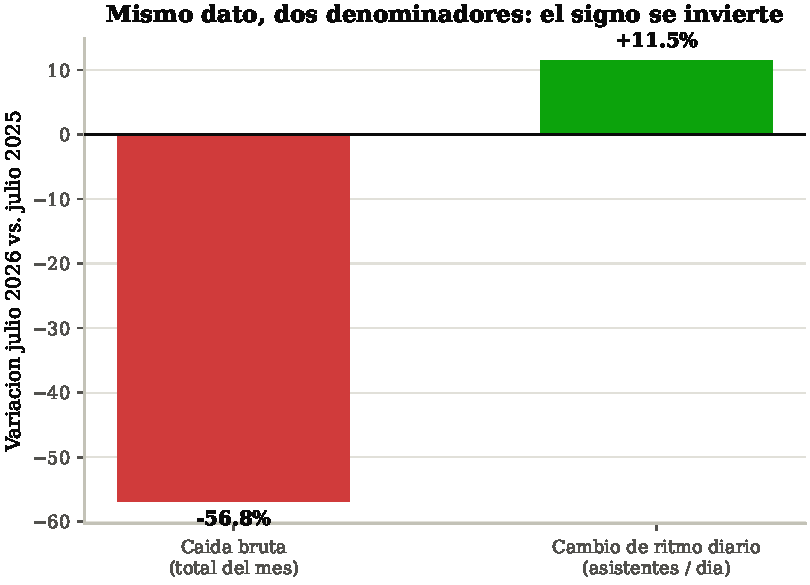
\includegraphics[width=0.85\linewidth]{caso3_q3_signo.pdf}
\caption{Mismo dato, dos denominadores: la caída bruta de julio (-56.8\%, comparando totales de mes con distinta exposición) se invierte a +11.5\% al comparar el ritmo diario (asistentes por día observado).}
\label{fig:c3-q3}
\end{figure}

\subsection{Pregunta 4 --- Comparar las 12 sedes}
\label{ssec:c3-q4}

\paragraph{Concepto técnico.}
Los pequeños múltiplos con \textbf{escala común} (mismo eje $Y$ en los 12 paneles) responden \enquote{¿qué sede aporta más volumen absoluto?} --- comparación de magnitud. Los pequeños múltiplos con \textbf{índice base 100} (cada sede reescalada a su propio valor de referencia) responden \enquote{¿qué sede creció, cayó o se recuperó en términos relativos?} --- comparación de forma/recuperación, independiente del tamaño. La segunda vista es la que se necesita cuando las sedes tienen tamaños muy distintos y un quiebre afecta solo a algunas \citep{munzner2014visualization}.
\[
\text{índice}_{t} = \frac{\text{asistentes}_t}{\text{asistentes}_{\text{ene-2025}}}\times100 .
\]

\paragraph{Evidencia.}
\textbf{Magnitud (escala común):} tamaño medio mensual 2025 --- Lima (SED-01) = 38\,557; Cusco (SED-06) = 23\,500; Arequipa (SED-05) = 22\,333; $\ldots$; Iquitos (SED-11) = 13\,037; Pucallpa (SED-12) = 11\,242 (la más pequeña). Lima es 3.4$\times$ más grande que Pucallpa: en una vista de escala común, la caída de Iquitos/Pucallpa durante el quiebre (a $\sim$7\,100--8\,518) queda visualmente aplastada contra un eje $Y$ dominado por Lima --- el quiebre casi no se nota.
\textbf{Recuperación relativa (índice base 100, ref. enero-2025):} Iquitos cae a 63.5 (mar-25) $\rightarrow$ 63.3 (abr-25) $\rightarrow$ 55.6 (may-25) y se recupera a 101.9 en jun-25, alcanzando 125.8 en jul-25 (estacionalidad) y 151.0 en dic-25 (pico). Pucallpa: 66.1 $\rightarrow$ 63.2 $\rightarrow$ 63.6, recupera 102.5 en jun-25 y 154.0 en dic-25. Lima, en la misma ventana, solo fluctúa por estacionalidad normal (106.4 en mar-25, 99.9 en abr-25, 112.9 en may-25, sin ningún \emph{dip}). El índice hace visible una \enquote{V} clara de caída y recuperación en 3 meses que la vista de escala común esconde por completo.

\paragraph{Decisión.}
Se mantiene 1 punto por mes $\times$ sede en ambas vistas --- sin agregar a trimestre o año --- con 12 paneles (uno por sede), eje $X$ = mes, ene-2024 a jul-2026. El quiebre se anota sin confundirlo con tendencia estructural: una banda sombreada entre 2025-03 y 2025-05, aplicada \emph{solo} en los paneles de Loreto y Ucayali, con la etiqueta explícita \enquote{Interrupción logística ficticia (evento puntual, 6/372 filas)} --- distinta de la banda de estacionalidad (jul/dic, que sí es recurrente y estructural). En 2026 ambas sedes vuelven a \enquote{Sin quiebre registrado}, confirmando que no es una tendencia nueva.

\paragraph{Límite / trade-off.}
El índice base 100 oculta la magnitud absoluta: una sede pequeña con alta variabilidad relativa puede parecer \enquote{más dramática} que Lima aunque mueva muchas menos personas en términos absolutos. Ninguna de las dos vistas reemplaza a la otra: se presentan una al lado de la otra, cada una etiquetada con la pregunta que responde.

La Figura~\ref{fig:c3-q4} indexa las 12 sedes a base 100 (ene-2025=100), resaltando Iquitos y Pucallpa sobre el resto en gris.

\begin{figure}[H]
\centering
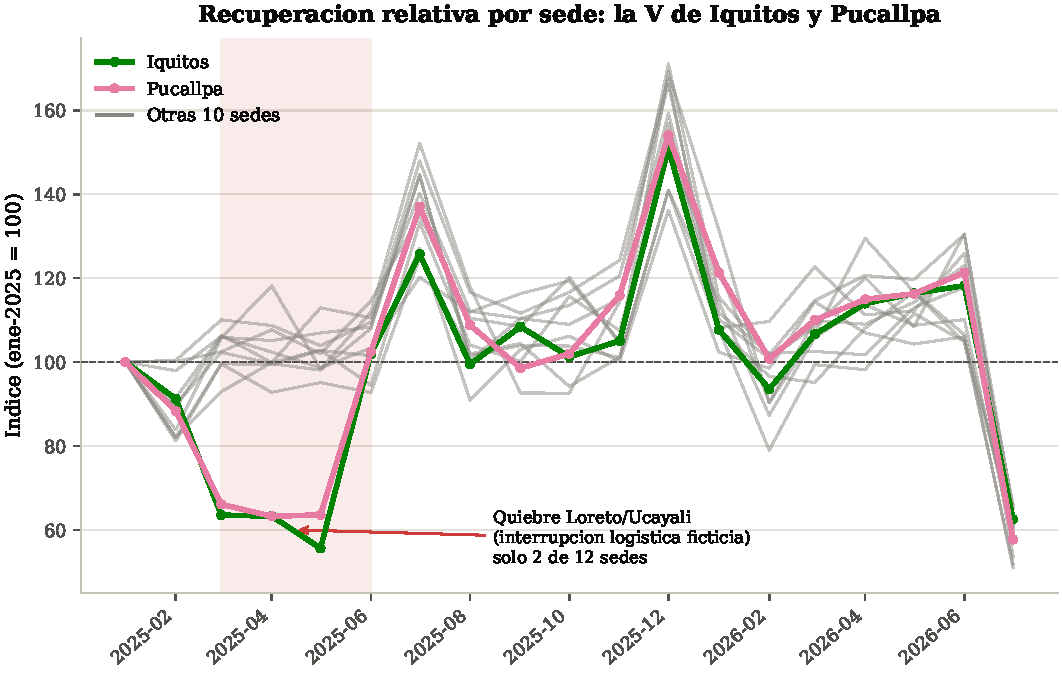
\includegraphics[width=0.85\linewidth]{caso3_q4_index.pdf}
\caption{Índice base 100 (ene-2025=100) por sede. Iquitos y Pucallpa (color) muestran la V de caída y recuperación del quiebre logístico (mar--may 2025); el resto de sedes (gris) solo fluctúa por estacionalidad, sin quiebre.}
\label{fig:c3-q4}
\end{figure}

\bitacora{Lima domina el festival; las demás sedes parecen estancadas o irrelevantes.}{Índice de recuperación post-quiebre, \(\text{índice}_t=(\text{asistentes}_t/\text{asistentes}_{\text{ene-2025}})\times100\); periodo mar--jun 2025; segmento Loreto (Iquitos, SED-11) y Ucayali (Pucallpa, SED-12); meta \(\text{índice}\ge100\) en junio-2025.}{Al indexar cada sede a base 100, Loreto y Ucayali muestran una V completa (63$\rightarrow$101 en 3 meses) que la vista de escala común, dominada por Lima, no deja ver.}{El quiebre fue real pero temporal; ambas sedes se recuperaron para junio-2025.}{El comité debería evaluar la resiliencia logística de Loreto/Ucayali (tiempo de recuperación) en vez de recortar presupuesto por \enquote{bajo desempeño} --- una decisión que solo emerge al mirar recuperación relativa y que la vista de magnitud absoluta, dominada por Lima, habría llevado a ignorar o mal-interpretar como debilidad estructural de la Selva.}

\paragraph{Síntesis del caso.}
Los cinco números ancla del enunciado se reproducen exactamente desde el CSV: total julio-2025 = 281\,044; total julio-2026 = 121\,281; cobertura julio-2026 = 38.71\%; caída bruta = -56.85\% ($\approx$ el titular -57\%); cambio de ritmo diario = +11.48\%. El hallazgo central es metodológico, no de negocio: el \enquote{colapso} de julio-2026 es un artefacto de comparar un mes truncado (12/31 días) contra un mes cerrado, no una caída real de asistencia. Corregido por cobertura, tanto el ritmo diario como el cumplimiento de meta (121\,281 / 120\,838 = 100.37\%) muestran a ChasquiFest por encima del año anterior.

\section{Caso 4 --- El mapa de la pasión que en realidad era el mapa del tamaño}
\label{sec:caso4}

El comité recibió un mapa de burbujas con asistencias \emph{absolutas} por sede: Lima tenía la burbuja mayor, el \textbf{diámetro} del símbolo se había escalado linealmente al valor (lo que distorsiona el \textbf{área} percibida) y el colormap \texttt{jet} pintaba una falsa ``montaña de intensidad''. El título concluía que Lima ``ama más'' al festival. Población, capacidad instalada y tasas normalizadas no llegaron a esa reunión, y sin ellas el comité no puede decidir dónde reforzar seguridad, dónde ampliar alcance ni dónde mejorar la experiencia.

\textbf{Granularidad del dataset:} una fila equivale a una sede/departamento del año 2025 (12 sedes, 12 eventos cada una). No existe una segunda columna de año, de modo que \textbf{todas} las comparaciones de este caso son intra-2025 (periodos homólogos por construcción; no se compara contra otro año porque el CSV no lo contiene).

Antes de rankear nada se verificaron las cuatro tasas ya provistas en el CSV: \texttt{alcance\_por\_1000\_hab}, \texttt{reclamos\_por\_10000\_asistencias}, \texttt{ocupacion\_pct} y \texttt{costo\_por\_asistente\_soles}. Recalculadas fila a fila como numerador/denominador, la diferencia máxima absoluta contra el valor publicado en el CSV fue menor a 0.01 en las cuatro (redondeo de fuente): quedan confirmadas como fórmulas explícitas, no como agregados opacos.

\subsection{Pregunta 1 --- Un ranking por decisión}
\label{ssec:c4-q1}

Cada decisión del comité necesita una métrica distinta, con un \textbf{denominador distinto}. Ninguna de las tres es ``la verdadera'': responden preguntas diferentes.

\textbf{(a) Volumen --- asignar personal de seguridad.}

\paragraph{Concepto técnico.} Aforo absoluto: conteo de asistencias, no de personas distintas. Mide carga operativa total a custodiar; no se normaliza porque la seguridad se dimensiona contra multitudes físicas reales, no contra tasas.

\paragraph{Evidencia.} Métrica \texttt{asistentes\_2025}; numerador = asistencias 2025, \textbf{denominador = ninguno} (magnitud absoluta, no una tasa). Los cinco primeros lugares: Lima 462\,690, Cusco 281\,998, Arequipa 268\,001, Trujillo 253\,960 y Piura 246\,920 (Tabla~\ref{tab:c4-rankings}, columna Volumen).

\paragraph{Decisión.} \textbf{Tableau:} \lstinline{SUM([asistentes_2025])} con \emph{table calc} \lstinline{RANK(SUM([asistentes_2025]))}. Partición: ninguna (la tabla completa; granularidad = 1 fila/sede, un solo año). \emph{Addressing}: Ciudad/Departamento (el ranking recorre esa dimensión). \textbf{pandas:} \lstinline{df['asistentes_2025'].rank(ascending=False)}.

\paragraph{Límite / trade-off.} Ignora la ocupación relativa del recinto. Tarapoto opera al \textbf{92.46\%} de su capacidad (156\,388/169\,146 = asistentes\_2025/capacidad\_anual\_2025) --- la ocupación más alta de las 12 sedes--- pero por volumen bruto cae al puesto \#9, recibiendo relativamente poco refuerzo si el criterio fuera solo volumen. Riesgo: sedes pequeñas casi llenas quedan sub-atendidas en seguridad.

\textbf{(b) Tasa poblacional --- comparar alcance territorial.}

\paragraph{Concepto técnico.} Penetración territorial: cuántas personas \emph{distintas} de la población de referencia fueron alcanzadas, normalizando por tamaño poblacional para comparar sedes de escala muy distinta.

\paragraph{Evidencia.}
\[
\texttt{alcance\_por\_1000\_hab} = \frac{\texttt{visitantes\_unicos\_2025}}{\texttt{poblacion\_referencial}} \times 1000
\]
(confirmado, diferencia máxima 0.0043 frente al recálculo). Numerador = visitantes únicos 2025; denominador = población referencial. Los cinco primeros: Cusco 157.89 (221\,678/1\,404\,000), Ayacucho 146.86 (98\,130/668\,200), Pucallpa 135.62 (87\,911/648\,200), Tarapoto 126.07 (117\,551/932\,400) y Arequipa 123.90 (202\,092/1\,631\,100). Lima cae al último lugar de las 12 sedes con \textbf{31.96} (324\,391/10\,151\,200).

\paragraph{Decisión.} \textbf{Tableau:} \lstinline{SUM([visitantes_unicos_2025])/SUM([poblacion_referencial])*1000}, con \lstinline{RANK(...)}. Partición: ninguna. \emph{Addressing}: Ciudad/Departamento. \textbf{pandas:} \lstinline{(df.visitantes_unicos_2025/df.poblacion_referencial*1000).rank(ascending=False)}.

\paragraph{Límite / trade-off.} Premia poblaciones chicas. Pucallpa (población 648\,200, la más pequeña de las 12) entra al podio de alcance, mientras Lima --- con 10\,151\,200 hab., 15.7 veces la población de Pucallpa--- queda relegada, aunque en términos absolutos deja sin cubrir a \textbf{9\,826\,809 personas (96.80\% de su población referencial)} que nunca asistieron en 2025. Ese mercado sin explotar no aparece en un ranking de tasas.

\textbf{(c) Tasa de reclamos --- priorizar calidad operativa.}

\paragraph{Concepto técnico.} Intensidad de fricción por unidad de actividad: normaliza reclamos por volumen de asistencia para comparar ``calidad percibida'' entre sedes de tamaño distinto.

\paragraph{Evidencia.}
\[
\texttt{reclamos\_por\_10000\_asistencias} = \frac{\texttt{reclamos\_totales}}{\texttt{asistentes\_2025}} \times 10000
\]
(confirmado, diferencia máxima 0.0046). Numerador = reclamos totales; denominador = asistencias 2025 (no visitantes únicos). Los cinco peores: Cusco 69.01 (1\,946/281\,998), Ayacucho 65.58 (973/148\,376), Piura 62.61 (1\,546/246\,920), Pucallpa 54.78 (739/134\,905) y Lima 42.92 (1\,986/462\,690).

\paragraph{Decisión.} \textbf{Tableau:} \lstinline{SUM([reclamos_totales])/SUM([asistentes_2025])*10000}, con \lstinline{RANK(...)} descendente (mayor tasa = peor). Partición: ninguna. \emph{Addressing}: Ciudad/Departamento. \textbf{pandas:} \lstinline{(df.reclamos_totales/df.asistentes_2025*10000).rank(ascending=False)}.

\paragraph{Límite / trade-off.} Puede castigar sedes con mejor cultura o mayor accesibilidad de canales de reporte (más fácil quejarse produce más reclamos registrados, no necesariamente peor servicio), o premiar sedes con canales pobres. Puno tiene la tasa más baja (18.41): no puede afirmarse causalmente que da mejor servicio --- podría tener menos canales de reporte (asociación, no causalidad). Dato de contexto: en Cusco solo el \textbf{16.70\%} de sus 1\,946 reclamos son de accesibilidad (\texttt{reclamos\_accesibilidad} = 325) --- el porcentaje más bajo de las 12 sedes--- lo que sugiere que su fricción no es solo de accesibilidad, aunque tampoco prueba causa-raíz sin investigación cualitativa adicional.

\begin{table}[H]
\centering
\small
\caption{Los cinco primeros lugares de cada ranking, 2025 (12 sedes). El líder cambia con el denominador.}
\label{tab:c4-rankings}
\begin{tabular}{c l l l}
\toprule
Puesto & Volumen (asistentes\_2025) & Alcance (/1\,000 hab.) & Reclamos (/10\,000 asist.) \\
\midrule
1 & Lima (462\,690) & Cusco (157.89) & Cusco (69.01) \\
2 & Cusco (281\,998) & Ayacucho (146.86) & Ayacucho (65.58) \\
3 & Arequipa (268\,001) & Pucallpa (135.62) & Piura (62.61) \\
4 & Trujillo (253\,960) & Tarapoto (126.07) & Pucallpa (54.78) \\
5 & Piura (246\,920) & Arequipa (123.90) & Lima (42.92) \\
\bottomrule
\end{tabular}
\end{table}

\textbf{Evidencia del reordenamiento.} Lima pasa de \#1 en volumen a \#12 (último lugar) en alcance y \#5 en reclamos; Cusco pasa de \#2 en volumen a \#1 en alcance \emph{y} \#1 en reclamos simultáneamente. Ninguno de los tres rankings es falso: miden objetivos distintos con denominadores distintos. Volumen (sin denominador) responde ``¿dónde hay más gente físicamente?''; alcance (denominador = población) responde ``¿qué proporción del territorio se activó?''; reclamos (denominador = asistencias) responde ``¿qué tan fricción-intensiva es la experiencia por visita?''. Lima domina el primero porque concentra el \textbf{41.05\%} de la población de referencia nacional (10\,151\,200/24\,729\,200) pero solo el \textbf{17.11\%} de las asistencias totales (462\,690/2\,703\,721): es grande en términos absolutos pero relativamente poco penetrada. Cusco lidera el segundo \emph{y} es alto en el tercero al mismo tiempo --- alta penetración y alta fricción no son contradictorias, son dos caras de una sede muy demandada relativa a su tamaño.

\begin{figure}[H]
\centering
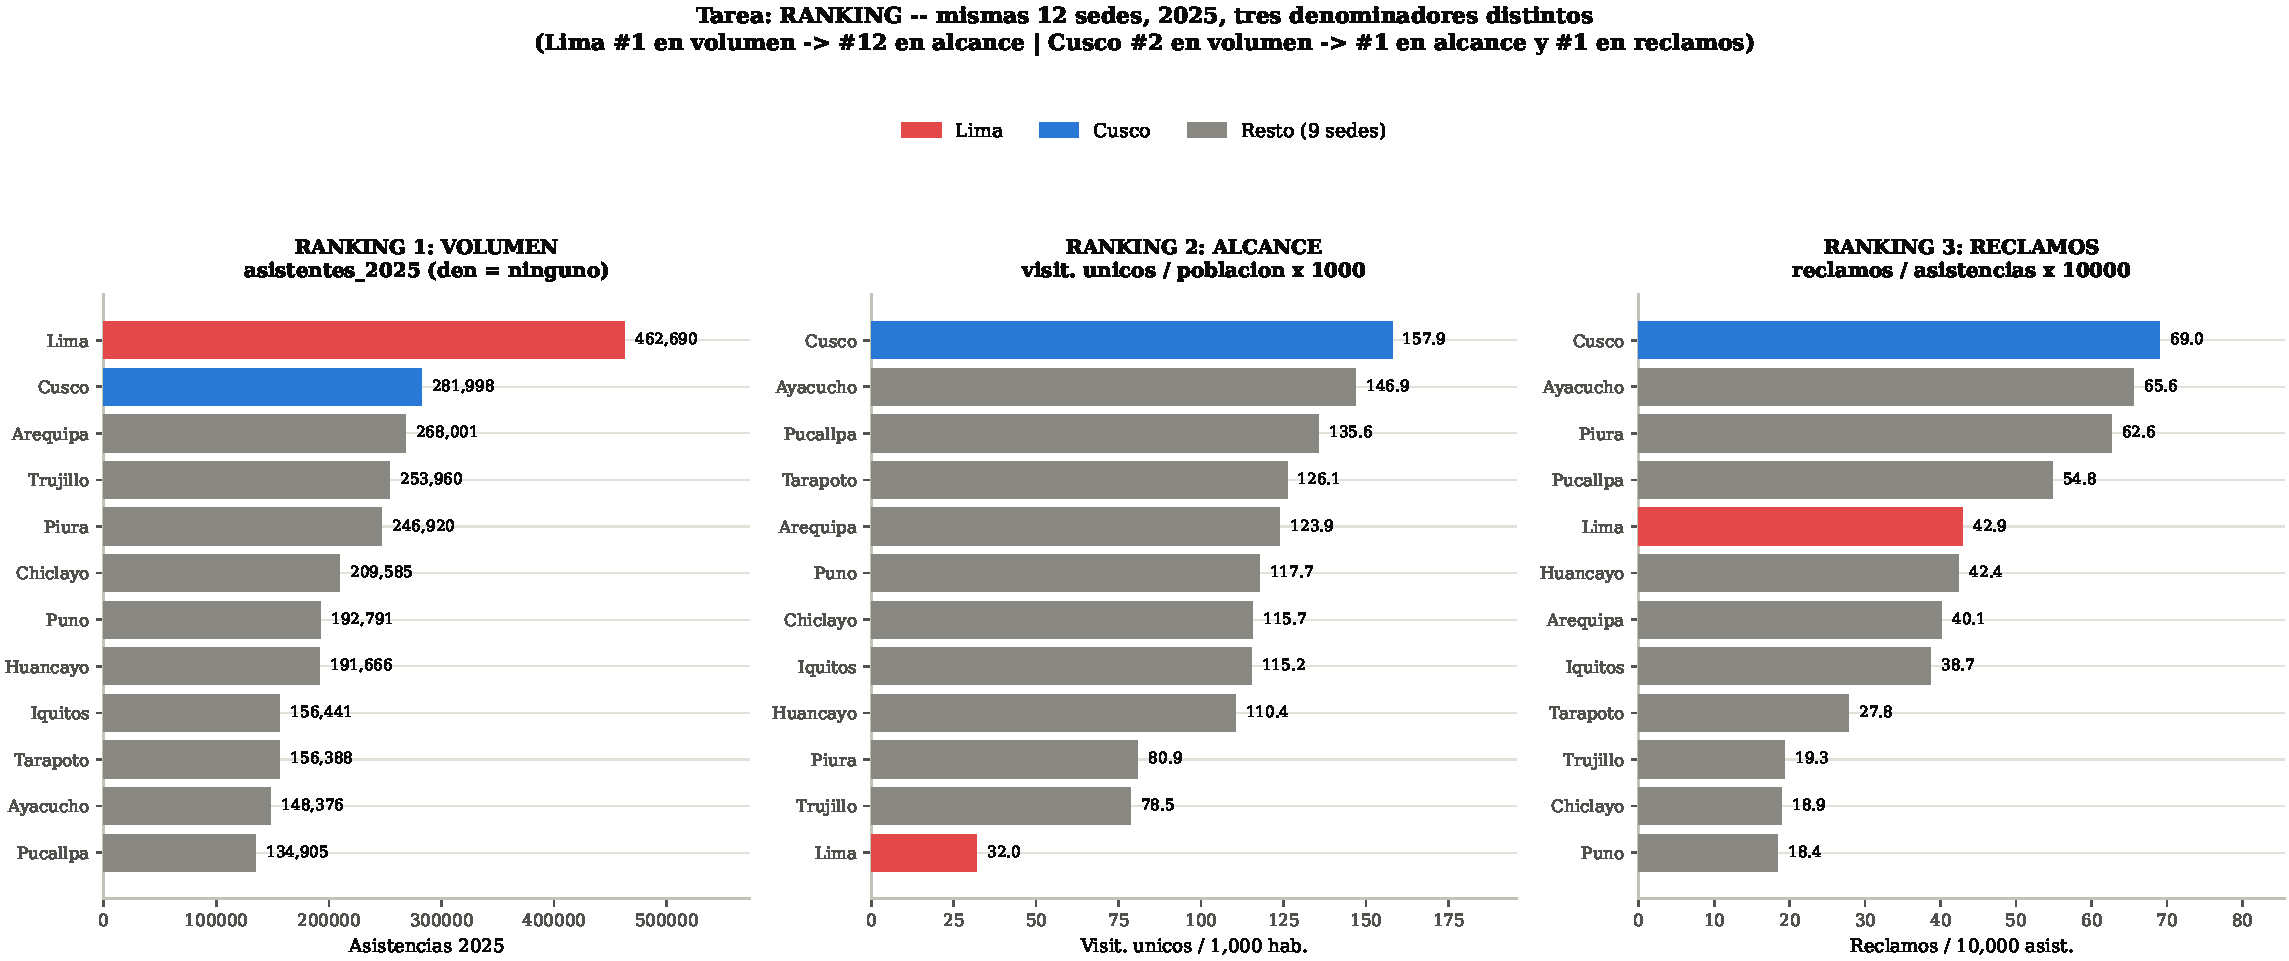
\includegraphics[width=0.98\linewidth]{caso4_q1_rankings.pdf}
\caption{Tarea analítica: \emph{ranking} / comparación de magnitud. Tres barras horizontales ordenadas, una por métrica, mismas 12 sedes. El canal usado es posición en eje --- el que Cleveland y McGill \citep{cleveland1984graphical} identifican como el más preciso para juicios de magnitud, muy superior a área o color. Lima (rojo) y Cusco (azul) se resaltan para visualizar el reordenamiento.}
\label{fig:c4-q1}
\end{figure}

\subsection{Pregunta 2 --- Mapa o barra}
\label{ssec:c4-q2}

\paragraph{Concepto técnico.} Dos preguntas distintas exigen dos tareas analíticas distintas, y cada tarea exige un tipo de gráfico distinto \citep{munzner2014visualization}. ``¿Dónde?'' exige un \textbf{mapa} (tarea: localización geográfica / distribución espacial), usando \texttt{latitud}/\texttt{longitud} para posicionar cada sede en su ubicación real: símbolos proporcionales (\emph{bubble map}) cuando la variable es un conteo/volumen absoluto (\texttt{asistentes\_2025}), porque el tamaño del símbolo codifica magnitud sin inflar el área del polígono territorial que ya de por sí varía por departamento; un coroplético \emph{normalizado} queda reservado para tasas por población o por actividad (\texttt{alcance\_por\_1000\_hab}, \texttt{reclamos\_por\_10000\_asistencias}, \texttt{ocupacion\_pct}), porque el color debe representar algo \emph{por unidad} de esa área o población, no un conteo bruto. ``¿Quién lidera y por cuánto?'' exige una \textbf{barra ordenada} (tarea: ranking / comparación de magnitud, canal = posición en eje): ordenar descendente por la métrica elegida, eje corto = categoría (sede), eje largo = valor, con etiquetas numéricas directas para lectura exacta (Figura~\ref{fig:c4-q1}).

\paragraph{Evidencia.} Si se pintara el departamento de Lima con el color más intenso solo por tener 462\,690 asistencias, el mapa terminaría mostrando ``dónde vive más gente'', no ``dónde el festival tuvo más impacto relativo''. Lima tiene 10\,151\,200 habitantes, el \textbf{41.05\%} de la población de referencia total (10\,151\,200/24\,729\,200); cualquier conteo bruto (asistentes, reclamos totales, costo público) se correlaciona mecánicamente con población, y las áreas grandes/pobladas ``ganan'' siempre en un coroplético de conteos, sin importar la variable. Dos titulares compiten por la atención del comité, y ambos son ciertos: \textbf{Volumen} --- ``Lima concentra 462\,690 asistencias, el mayor aforo'' (Ranking 1, P1a); \textbf{Alcance} --- ``Cusco alcanza 158 visitantes por mil habitantes, el mayor alcance por habitante'' (Ranking 2, P1b).

\paragraph{Decisión.} Cada titular apunta a un recurso distinto del comité; no son intercambiables. Volumen $\rightarrow$ reforzar personal de seguridad y logística de multitudes en Lima (Pregunta 1a): responde a carga física absoluta, sin denominador. Alcance $\rightarrow$ estudiar la experiencia y calidad de servicio en Cusco (Pregunta 1c), no necesariamente expandir infraestructura física: responde a penetración relativa a la población, no a volumen. La Figura~\ref{fig:c4-q2} implementa el mapa correcto: área del símbolo $\propto$ \texttt{asistentes\_2025} y color en \texttt{viridis} sobre \texttt{alcance\_por\_1000\_hab}, con la barra ordenada de la Figura~\ref{fig:c4-q1} como vista de soporte para el ranking.

\paragraph{Límite / trade-off.} Una tasa alta no es evidencia de causa ni de afecto --- el mismo error que decir ``Cusco ama más''. La \texttt{ocupacion\_pct} de Cusco es \textbf{74.96\%}, la más baja de las 12 sedes, de modo que el alto alcance y la alta tasa de reclamos de Cusco (69.01, Pregunta 1c) \textbf{no} se explican por saturación física del recinto (no está ``lleno''); apuntan más bien a gestión de flujos, servicios o accesibilidad, algo que solo una investigación cualitativa adicional podría confirmar. ``Mayor alcance por habitante'' describe una tasa de penetración territorial, no un sentimiento de apego: inferir ``arraigo'' o ``amor'' a partir de \texttt{alcance\_por\_1000\_hab} cometería el mismo salto lógico (tasa $\rightarrow$ causa/afecto) que el titular original del mapa de burbujas.

\begin{figure}[H]
\centering
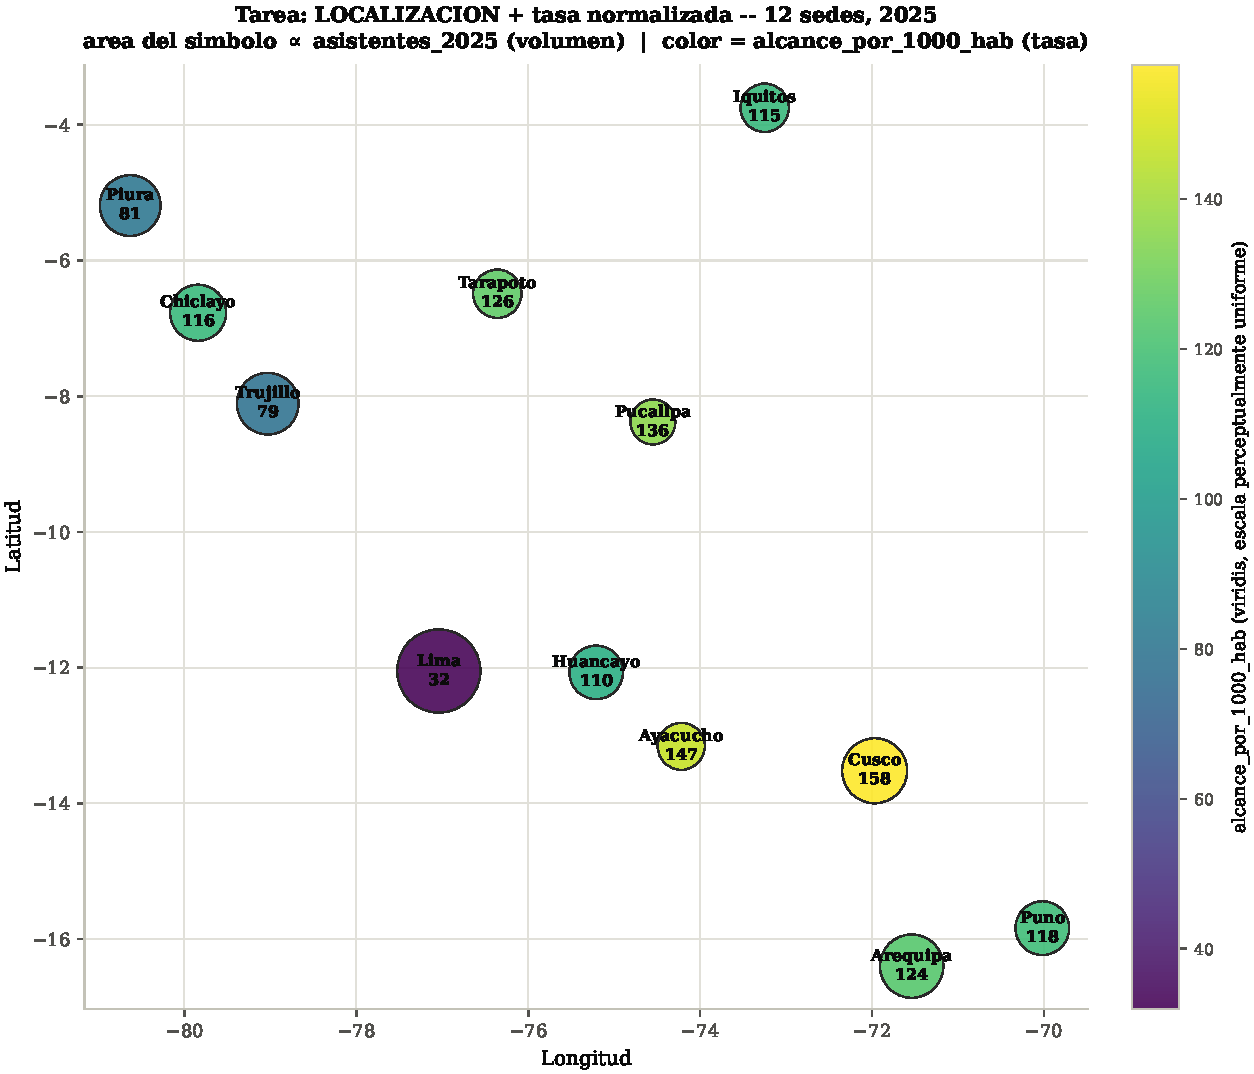
\includegraphics[width=0.85\linewidth]{caso4_q2_mapa.pdf}
\caption{Tarea analítica: localización geográfica + tasa normalizada. Las 12 sedes posicionadas por \texttt{latitud}/\texttt{longitud}; área del símbolo $\propto$ \texttt{asistentes\_2025} (volumen absoluto); color \texttt{viridis} sobre \texttt{alcance\_por\_1000\_hab} (tasa), con la etiqueta numérica directa del valor de alcance sobre cada sede como canal redundante al color. Lima es la burbuja más grande y, a la vez, la de color más oscuro (menor alcance); Cusco es una burbuja mediana pero la más clara (mayor alcance).}
\label{fig:c4-q2}
\end{figure}

\subsection{Pregunta 3 --- Área, color y acceso}
\label{ssec:c4-q3}

\paragraph{Concepto técnico.} El error clásico de ``burbuja mal escalada''. Si el \textbf{diámetro} se escala linealmente al valor, el \textbf{área} --- lo que el ojo realmente integra al leer un círculo \citep{cleveland1984graphical} --- crece con el \textbf{cuadrado} del valor, exagerando visualmente las diferencias.

\paragraph{Evidencia.} Con números reales: Lima (462\,690 asistentes) frente a Pucallpa (134\,905 asistentes), razón de valores
\[
r = \frac{462\,690}{134\,905} = 3.4297\times.
\]
Con diámetro $\propto$ valor: razón de diámetros = $r = 3.4297\times$, pero razón de \textbf{áreas} = $r^2 = 11.7632\times$. El área de la burbuja de Lima aparece \textbf{11.76 veces} más grande que la de Pucallpa aunque el dato real es solo \textbf{3.43 veces} mayor --- una sobre-representación visual adicional de exactamente $r^2/r = r = 3.4297\times$.

\paragraph{Decisión.} Escalar por \textbf{área}, no por diámetro:
\[
\text{área} \propto \text{valor} \;\Longleftrightarrow\; \text{diámetro} \propto \sqrt{\text{valor}}.
\]
Con esta corrección, razón de diámetros = $\sqrt{r} = 1.8520\times$, razón de áreas = $(\sqrt{r})^2 = 3.4297\times$, que coincide exactamente con la razón real de asistencias. \textbf{Tableau:} en el estante \emph{Size}, Tableau ya escala por defecto el \textbf{área} del símbolo (no el diámetro) al soltar un campo continuo --- el error típicamente ocurre en herramientas o código que fijan \texttt{markersize}/\texttt{radius} de forma lineal. \textbf{pandas/matplotlib:}
\begin{lstlisting}[style=cod]
s = k * valor   # plt.scatter interpreta 's' como AREA en puntos^2: correcto
markersize = k * valor  # plt.plot: markersize es DIAMETRO lineal -> error equivalente
\end{lstlisting}

\paragraph{Límite / trade-off.} Incluso corregido por área, el ojo humano \textbf{subestima} áreas grandes (compresión de Stevens, exponente $\approx 0.7$ para área), así que ningún \emph{bubble map} da lectura cuantitativa exacta; por eso debe acompañarse siempre de una etiqueta numérica directa o de una barra ordenada (canal de posición) para lectura precisa.

\textbf{Reemplazo de colormap.} \texttt{jet} no es perceptualmente uniforme: su luminancia no es monótona, crea falsos bordes/bandas de contorno que no corresponden a discontinuidades reales en los datos, y no es legible en escala de grises ni amigable para daltonismo rojo-verde (deuteranopía/protanopía). Reemplazo: \textbf{viridis} (o \textbf{cividis}, optimizado específicamente para deuteranopía) --- luminancia monótonamente creciente, perceptualmente uniforme en CIELAB, legible en escala de grises.

\textbf{Dos canales redundantes} (mantienen la lectura con daltonismo o en escala de grises, sin depender del color, presentes en la Figura~\ref{fig:c4-q2}): (1)~etiqueta numérica directa sobre cada símbolo con el valor de \texttt{alcance\_por\_1000\_hab} (p. ej. ``Cusco 158''), que permite leer exactamente la variable codificada en color sin decodificar el tono; (2)~tamaño/área del símbolo ($\propto$ \texttt{asistentes\_2025}) como segundo canal, ordinal y perceptible incluso en escala de grises, que separa visualmente a Lima del resto sin necesitar distinguir colores.

\begin{figure}[H]
\centering
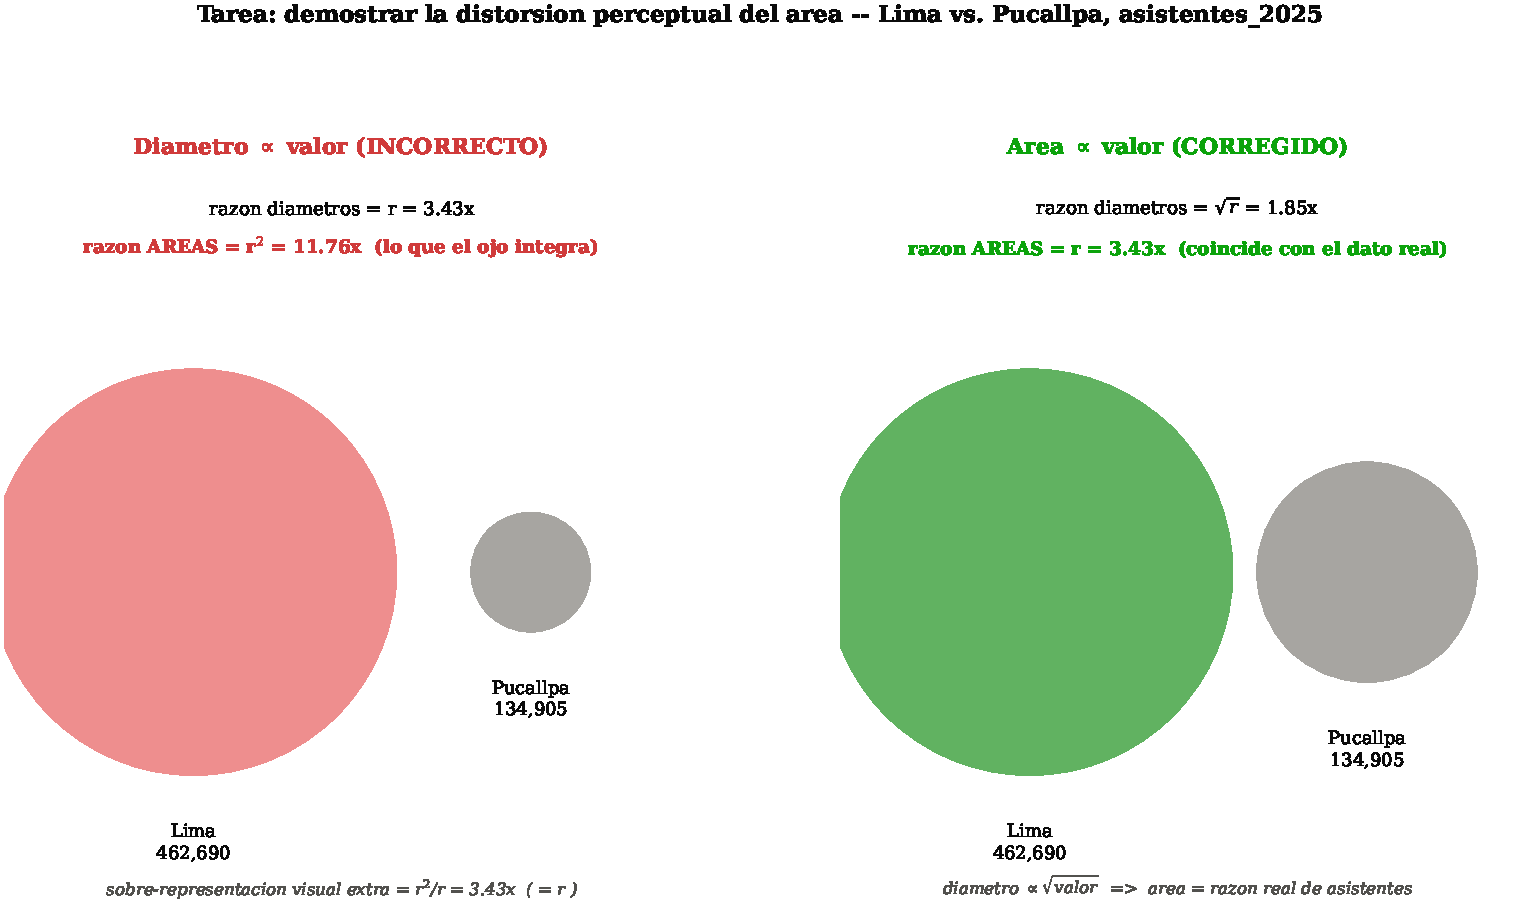
\includegraphics[width=0.9\linewidth]{caso4_q3_distorsion.pdf}
\caption{Demostración numérica de la distorsión diámetro-vs-área, Lima vs. Pucallpa (\texttt{asistentes\_2025}). Izquierda: diámetro $\propto$ valor (incorrecto), el área aparente exagera la razón real en un factor $r$ adicional. Derecha: área $\propto$ valor (corregido), el área aparente coincide exactamente con la razón real de asistencias.}
\label{fig:c4-q3}
\end{figure}

\subsection{Pregunta 4 --- Dashboard de decisión}
\label{ssec:c4-q4}

\paragraph{Concepto técnico.} Un dashboard de decisión reemplaza el mapa único por una vista compuesta: una franja de KPI con estado semáforo, una vista principal de localización (mapa corregido), una vista de soporte de ranking (barra ordenada) y un panel de insights textuales, todo con el mismo periodo, segmento y fuente declarados.

\paragraph{Evidencia.} Los cuatro KPI nacionales de 2025 se agregan como \textbf{ratio-de-sumas} ($\mathrm{SUM(num)}/\mathrm{SUM(den)}$), no como promedio-de-tasas, para evitar el sesgo de ponderación por tamaño de sede \citep{gelman2007average}: la ocupación agregada nacional es \textbf{83.89\%} (2\,703\,721/3\,222\,747) frente al promedio simple de \texttt{ocupacion\_pct} por sede de \textbf{84.75\%} --- no son lo mismo, porque el promedio simple pondera igual a Pucallpa (capacidad 146\,046) que a Lima (capacidad 556\,171). En Tableau esto se expresa con un LOD fijo:
\begin{lstlisting}[style=cod]
{FIXED : SUM([reclamos_totales])/SUM([asistentes_2025])*10000}   // ratio-de-sumas, correcto
AVG([reclamos_por_10000_asistencias])                            // promedio de tasas, NO equivalente
\end{lstlisting}

\begin{table}[H]
\centering
\small
\caption{Los cuatro KPI del dashboard, 2025 (agregado nacional = ratio-de-sumas). Meta = benchmark interno (mediana de las 12 sedes), declarado por este análisis; el CSV no trae una meta oficial del comité.}
\label{tab:c4-kpi}
\begin{tabularx}{\linewidth}{@{}>{\raggedright\arraybackslash}p{1.9cm} >{\raggedright\arraybackslash\ttfamily\scriptsize}p{5.2cm} >{\raggedright\arraybackslash}X >{\raggedright\arraybackslash}p{2.3cm}@{}}
\toprule
Rol & KPI (fórmula) & Valor 2025 (num./den.) & Estado (brecha) \\
\midrule
RESULTADO & asistentes\_2025 / capacidad\_anual\_2025 $\times$100 & 83.89\% (2\,703\,721/3\,222\,747); meta $\geq 85\%$ & AMARILLO ($-1.11$ pp) \\
EFICIENCIA & costo\_publico\_soles / asistentes\_2025 & S/~14.03; meta $\leq$ S/~13.64 (mediana) & ROJO ($+2.84\%$) \\
RIESGO & reclamos\_totales / asistentes\_2025 $\times$10000 & 42.02; meta $\leq 41.27$ (mediana) & ROJO/ALERTA ($+1.83\%$) \\
ALCANCE/\newline EQUIDAD & visitantes\_unicos\_2025 / poblacion\_referencial $\times$1000 & 79.58; meta $\geq 116.67$ (mediana) & ROJO ($-31.79\%$) \\
\bottomrule
\end{tabularx}
\end{table}

\paragraph{Decisión.} Cada tarjeta enlaza directamente con una acción. \textbf{RESULTADO} (AMARILLO): revisar programación y franjas horarias en sedes con capacidad ociosa para cerrar la brecha de $-1.11$ pp hacia la meta. \textbf{EFICIENCIA} (ROJO): auditar y renegociar costos logísticos en las sedes sobre la mediana (máximo Chiclayo, S/~18.56/asistente; mínimo Piura, S/~9.72/asistente) para converger a S/~13.64/asistente. \textbf{RIESGO} (ROJO/ALERTA): reforzar atención al público y protocolos de accesibilidad en las cuatro sedes de la zona crítica (tasa $>50$/10\,000): Cusco (69.01), Ayacucho (65.58), Piura (62.61) y Pucallpa (54.78), en ese orden de prioridad. \textbf{ALCANCE/EQUIDAD} (ROJO): priorizar campañas de difusión y nuevas franjas o sedes en departamentos bajo la mediana de alcance (brecha $-31.79\%$).

Ejemplo de tarjeta completa (RIESGO, la más ligada a seguridad/experiencia): \textbf{valor} 42.02 reclamos por cada 10\,000 asistencias; \textbf{periodo} 2025 (año completo, 12 eventos por sede; único periodo disponible en el CSV, no se compara con otro año); \textbf{segmento} las 12 sedes/departamentos (agregado nacional = ratio-de-sumas); \textbf{comparación/meta} mediana de sedes = 41.27 (línea de referencia), meta operativa propuesta $\leq 40.00$ (declarada por este análisis, límite explícito, no viene en el CSV); \textbf{estado} semáforo ROJO/ÁMBAR; \textbf{acción} asignar equipos de atención al público y revisar protocolos de accesibilidad en Cusco, Ayacucho, Piura y Pucallpa, en ese orden (orden = magnitud de la tasa, no del volumen absoluto).

El \textbf{layout} (1280$\times$720~px, cinco filas) coloca: (1)~título-pregunta; (2)~franja de 4 tarjetas KPI con estado semáforo; (3)~vista principal a la izquierda ($\sim$800~px) con el mapa de símbolos proporcionales de la Figura~\ref{fig:c4-q2} (tarea: localización) y vista de soporte a la derecha ($\sim$450~px) con la barra ordenada configurable de la Figura~\ref{fig:c4-q1} (tarea: ranking); (4)~panel de insights con tres números clave (Lima: 41.05\% de la población, 17.11\% de las asistencias, alcance 31.96/1\,000; Cusco: alcance \#1 y reclamos \#1 con ocupación 74.96\%, la más baja, luego no es saturación física; cuatro sedes en zona crítica de reclamos); (5)~pie metodológico con fuente, periodo y fórmulas de cada tasa. La jerarquía visual usa tamaño de fuente descendente título $>$ valor-KPI $>$ etiqueta; cada tarjeta agrupa valor, meta y estado en un solo bloque con espaciado uniforme (proximidad); las cuatro tarjetas comparten tipografía y fondo neutro (similitud), con el color de estado como único acento cromático variable, de modo que el ojo va directo a los dos rojos y un ámbar antes de leer cualquier número.

\paragraph{Límite / trade-off.} Las metas de ``mediana de las 12 sedes'' son un benchmark interno declarado por este análisis, no una meta oficial del comité; se documentan como límite explícito en vez de inventarse un objetivo externo. Además, el agregado nacional de alcance (79.58) queda muy por debajo de la mediana no ponderada de sedes (116.67) precisamente porque está ponderado por la población de Lima, que es enorme y de bajo alcance: un mismo número (79.58) resume sedes con realidades muy distintas y puede ocultar, otra vez, el mismo problema de agregación que motivó esta auditoría.

\bitacora{``Lima domina el festival; hay que reforzar Lima.'' (8 palabras)}{RESULTADO --- ocupación agregada nacional = \texttt{SUM(asistentes\_2025)} / \texttt{SUM(capacidad\_anual\_2025)} $\times$100, periodo 2025, segmento = 12 sedes, meta $\geq 85\%$ $\rightarrow$ valor real 83.89\%.}{Al normalizar por población (\texttt{alcance\_por\_1000\_hab}) y por asistencia (\texttt{reclamos\_por\_10000\_asistencias}), Cusco y Ayacucho emergen como focos de intensidad y fricción que el mapa de burbujas absolutas escondía detrás del tamaño de Lima.}{``Lima requiere volumen; Cusco y Ayacucho requieren calidad de experiencia.'' (10 palabras)}{El comité reasigna presupuesto: seguridad y logística escalan con volumen en Lima, mientras personal de atención y accesibilidad se refuerzan en Cusco, Ayacucho, Piura y Pucallpa según su tasa de reclamos, no según su tamaño.}

\section{Caso 5 --- Killa, el algoritmo y el juicio final}\label{sec:caso5}

\textbf{Afirmación bajo auditoría:} \emph{``Killa causó el boom: +108\% de ventas tras el video (15-abr), confirmado por un scatter vistas$\leftrightarrow$entradas con línea de tendencia''}. La tabla que sostiene esta afirmación tiene granularidad fecha$\times$sede (1\,464 filas = 122 días $\times$ 12 sedes, sin nulos, del 1-mar al 30-jun 2026); la campaña se divide en fase PRE (``Antes del video'', $n=540$) y fase POST (``Después del video'', $n=924$), con el video lanzado el 15-abr-2026. El titular ``+108\%'' ya tiene un primer problema de base de cálculo no declarada: sobre \texttt{ventas\_soles} la diferencia ingenua es +100.3\% (num$=7\,689.9-3\,839.6$, den$=3\,839.6$), no +108\%; el +108.2\% exacto (num$=225.25-108.21=117.04$, den$=108.21$) aparece recién al aplicar la misma cuenta sobre \texttt{entradas\_vendidas} (tickets). El dashboard mezcla soles y tickets sin decirlo --un problema independiente del problema de causalidad que se audita a continuación.

\subsection{Pregunta 1 --- Explorar no es explicar}\label{ssec:c5-q1}

\paragraph{Concepto técnico.} Un producto \emph{exploratorio} (muchos filtros, vistas alternativas, para que un analista busque patrones) y un producto \emph{explicativo} (una sola pregunta gobernando el diseño, para que un comité decida) responden a objetivos distintos. El dashboard de Killa tiene forma exploratoria --filtros de sobra, un scatter con línea de tendencia sin controles, una torta de vanidad-- pero se presenta como si ya respondiera la pregunta de negocio. Esa mezcla, no un detalle estético, es el problema de fondo.

\paragraph{Evidencia.} El mockup ofrece filtros de \texttt{sede}, \texttt{ciudad}, \texttt{macrozona}, \texttt{fecha}, \texttt{lluvia}, \texttt{promo}, \texttt{fin de semana}, \texttt{canal}, \texttt{color favorito} y \texttt{horóscopo}; un scatter ``más vistas = más entradas'' que cruza \texttt{vistas\_video\_miles} con \texttt{entradas\_vendidas} sin particionar por \texttt{festival\_abierto\_flag}, \texttt{inversion\_publicitaria\_soles} ni \texttt{promocion\_activa\_flag} (al introducir esos controles la $R^2$ cruda cae de 0.283 a $\sim$0.040, sección~\ref{ssec:c5-q3}); y una torta ``¿quién ama más a Killa?'' que no responde ninguna pregunta operativa.

\paragraph{Decisión.} Se retiran dos elementos de la entrega explicativa al comité: (1) los filtros de ``color favorito'' y ``horóscopo'', que no son variables de negocio ni existen en el CSV como impulsores de ventas y solo invitan a buscar un corte que ``confirme'' la historia; y (2) el scatter exploratorio vistas$\leftrightarrow$entradas con línea de tendencia, que induce a leer causalidad donde solo hay covariación con confusores comunes. Se reemplaza por la Figura~\ref{fig:c5-q3} (cruda vs. parcial), honesta sobre la incertidumbre. La torta ``¿quién ama más a Killa?'' también se retira: es un indicador social, no de negocio. La pregunta única que debe gobernar la versión explicativa es: \emph{¿el video generó ventas incrementales suficientes por sol invertido, una vez separado su efecto de la apertura de sedes, la inversión publicitaria y las promociones, como para justificar ampliar la campaña ahora?}

Clasificando las métricas del dashboard en la jerarquía actividad~$\to$~resultado~$\to$~impacto: \texttt{vistas\_video\_miles} es \textbf{actividad} (KPI de vanidad, mide exposición al contenido y sube 3.25$\times$ PRE$\to$POST, pero su relación cruda con ventas se explica en gran parte por confusores compartidos); \texttt{entradas\_vendidas} y \texttt{ventas\_soles} son \textbf{resultado} (comportamiento agregado, sin descontar causas); las ventas incrementales por sol invertido, controlando apertura, inversión y promoción, son el único candidato a \textbf{impacto} --y hoy, con datos observacionales, no se pueden estimar de forma confiable (sección~\ref{ssec:c5-q2}).

\paragraph{Límite / trade-off.} Reducir filtros y retirar el scatter libre le quita al comité la capacidad de explorar los datos por su cuenta, pero esa misma libertad fue lo que permitió la lectura causal errónea. Un producto explicativo sacrifica exploración a cambio de una conclusión defendible; si el comité necesita explorar, debe hacerlo en un \emph{workbook} aparte, no en la pantalla de decisión.

\subsection{Pregunta 2 --- Método científico y causalidad}\label{ssec:c5-q2}

\paragraph{Concepto técnico.} El método científico exige recorrer pregunta $\to$ hipótesis $\to$ datos $\to$ prueba $\to$ decisión sin saltarse pasos, y en particular sin confundir \emph{asociación observacional} --lo único que un CSV histórico puede mostrar sin experimento-- con \emph{causalidad} --lo que exigiría manipular el tratamiento (el video) de forma independiente del resto de factores.

\paragraph{Evidencia --- cadena método completa.}
\begin{enumerate}
  \item \textbf{Pregunta:} ¿el lanzamiento del video de Killa incrementó las ventas de entradas del festival?
  \item \textbf{Hipótesis (H1):} el video causó un aumento neto de ventas, más allá de lo explicado por apertura de sedes, inversión, promociones y estacionalidad. \textbf{Hipótesis nula (H0):} el aumento observado se explica total o mayormente por factores que cambiaron a la vez que el video.
  \item \textbf{Datos:} \texttt{caso5\_campania\_killa\_chasquifest.csv}, 1\,464 filas fecha$\times$sede, 1-mar a 30-jun 2026, video el 15-abr.
  \item \textbf{Prueba:} la diferencia bruta PRE/POST sobre \texttt{ventas\_soles} es num$=7\,689.9-3\,839.6=3\,850.3$, den$=3\,839.6$ $\to$ \textbf{+100.3\%} ($n_{\text{PRE}}=540$, $n_{\text{POST}}=924$). Restringiendo a sedes ya abiertas (\texttt{festival\_abierto\_flag}$=1$): num$=7\,956.2-9\,130.3=-1\,174.2$, den$=9\,130.3$ $\to$ \textbf{-12.9\%} ($n_{\text{PRE}}=206$, $n_{\text{POST}}=891$). Una regresión de \texttt{ventas\_soles} sobre \texttt{post} más los confusores observados confirma la inestabilidad: el coeficiente de \texttt{post} pasa de $+3\,850$ soles (modelo ingenuo, todas las sedes) a $-5\,185$ soles (con controles), y de $-1\,174$ soles (solo sedes abiertas, sin controles) a $-6\,460$ soles (solo sedes abiertas, con controles).
  \item \textbf{Decisión:} con los datos observacionales disponibles \textbf{no se rechaza H0}: no hay evidencia robusta de un efecto neto positivo del video una vez controlados los confusores observados. No es posible afirmar que ``Killa causó el boom''.
\end{enumerate}

\paragraph{Confusores identificados (media PRE $\to$ POST).}
\begin{table}[H]
\centering
\caption{Balance de confusores entre fase PRE y fase POST.}
\label{tab:c5-confusores}
\begin{tabular}{@{}lrrr@{}}
\toprule
Variable & PRE & POST & Cambio \\
\midrule
\texttt{festival\_abierto\_flag} (8$\to$12 sedes) & 0.38 & 0.96 & $+0.58$ \\
\texttt{inversion\_publicitaria\_soles} & 253.70 & 731.53 & $\times 2.88$ \\
\texttt{promocion\_activa\_flag} & 0.00 & 0.54 & solo existe en POST \\
\texttt{vistas\_video\_miles} & 5.51 & 17.89 & $\times 3.25$ \\
\texttt{fin\_de\_semana\_flag} (placebo) & 0.29 & 0.29 & $\approx 0$ \\
\bottomrule
\end{tabular}
\end{table}

Cuatro confusores se mueven junto con la fase de campaña: la apertura de sedes nuevas (8 de 12 sedes ya operaban en PRE, las 12 en POST --el promedio POST incluye sedes que no existían en PRE--), la inversión publicitaria (casi triplicada), las promociones (inexistentes antes del video, colinealidad casi perfecta con la fase) y, de forma adicional, la apertura escalonada de sedes entre el 1-mar y el 2-may --una sede (SED-09) abre exactamente el 15-abr, coincidencia temporal que refuerza visualmente la narrativa sin ser evidencia causal. En cambio \texttt{fin\_de\_semana\_flag} (0.29$\to$0.29) y \texttt{lluvia\_flag} (0.27$\to$0.27) no están confundidos y sirven de control de que el resto del diseño del CSV es razonable (Figura~\ref{fig:c5-q2a}).

\begin{figure}[H]\centering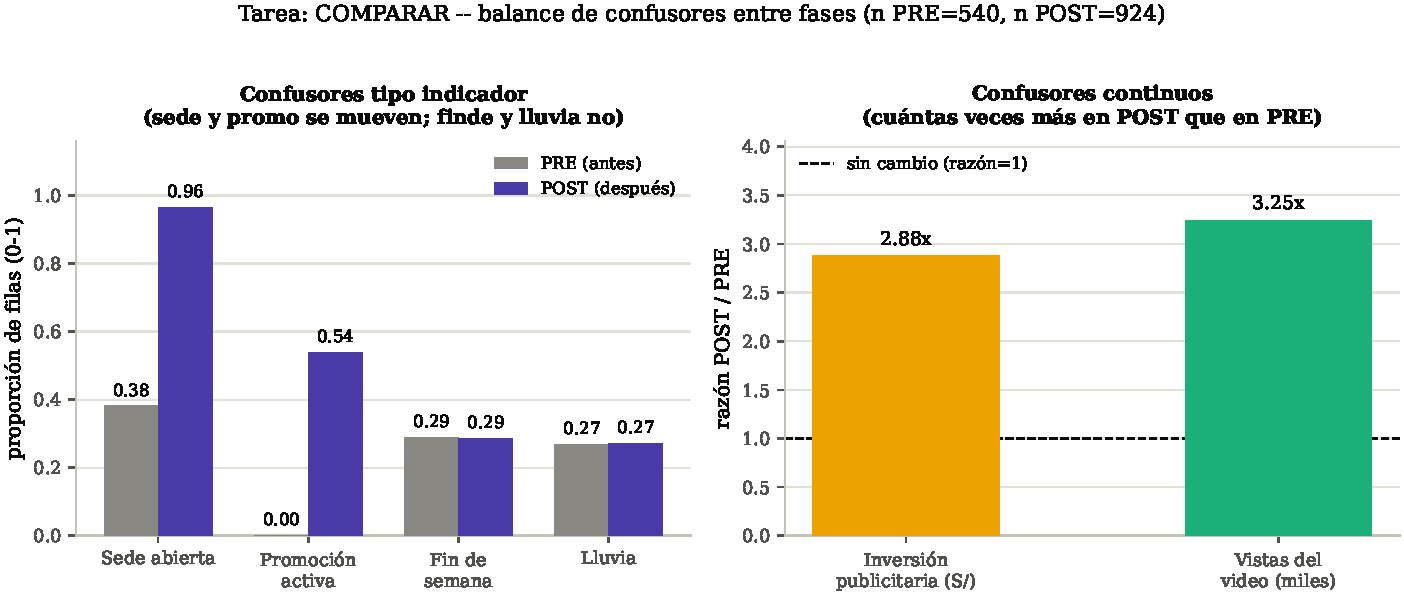
\includegraphics[width=0.95\linewidth]{caso5_q2_confusores.pdf}\caption{Balance de confusores PRE vs.\ POST: casi todo se mueve junto con la fase de campaña salvo fin de semana y lluvia.}\label{fig:c5-q2a}\end{figure}

Fijar la población de sedes invierte el signo de la diferencia bruta (Figura~\ref{fig:c5-q2b}):

\begin{figure}[H]\centering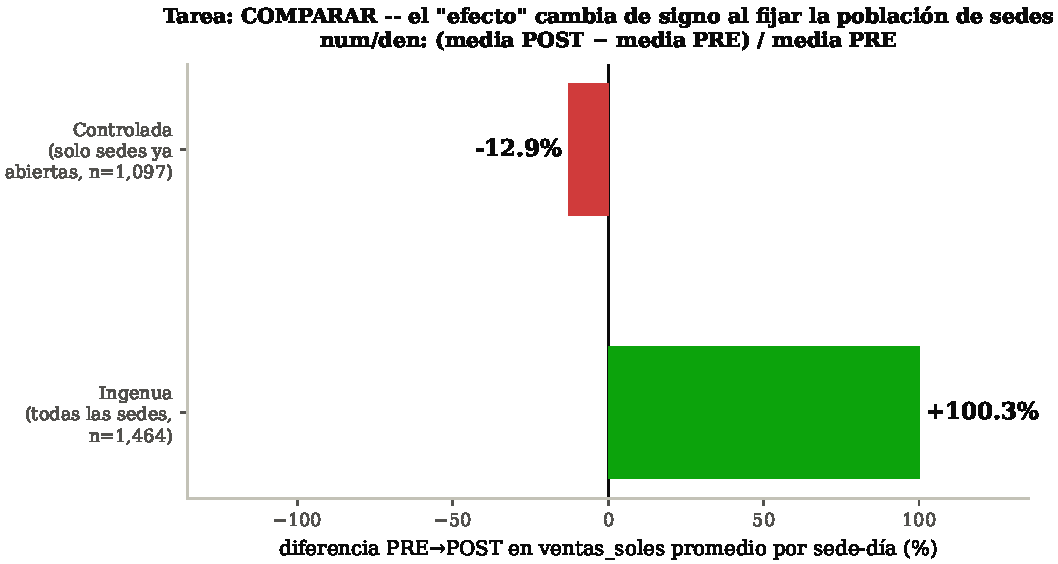
\includegraphics[width=0.85\linewidth]{caso5_q2_efecto.pdf}\caption{El ``efecto'' ingenuo (+100.3\%) se invierte a $-12.9$\% al controlar la apertura de sedes.}\label{fig:c5-q2b}\end{figure}

\paragraph{Decisión.} Se proponen dos diseños más fuertes, complementarios: (A) \emph{despliegue escalonado} (\emph{stepped-wedge}) por sede --dado que las 12 sedes ya abren en fechas distintas, un cronograma de intensificación de campaña aleatorizado en el tiempo por sede permitiría que cada sede sea control de sí misma antes de recibir el ``empujón'', separando el video del calendario de apertura e inversión-- y (B) una comparación tipo \emph{diferencias en diferencias}:
\begin{equation*}
\begin{aligned}
\texttt{ventas\_soles} \sim{} & \texttt{post} + \texttt{sede\_FE} + \texttt{tendencia\_fecha} \\
& + \texttt{inversion} + \texttt{promo} + \texttt{festival\_abierto}
\end{aligned}
\end{equation*}
con efectos fijos de sede y tendencia temporal, restringida a sedes abiertas todo el período --aproximada por el modelo controlado de sedes abiertas ($-6\,460$ soles), con la limitación honesta de que persiste sesgo de selección de sede. El umbral de decisión, definido antes de mirar el resultado: ampliar la campaña únicamente si las ventas incrementales por sol invertido en campaña son $\geq$ S/3 por sol, con intervalo de confianza al 95\% que excluya el cero, medido bajo un diseño controlado. Con los coeficientes disponibles (negativos pero no causalmente limpios) ese umbral queda \textbf{sin evaluar}, no alcanzado ni descartado.

\paragraph{Límite / trade-off.} Ni el modelo controlado ni la comparación intra-sedes-abiertas resuelven el confusor de ``cuáles sedes'': las sedes que abrieron antes probablemente son mercados más grandes o maduros, de modo que incluso restringiendo a ``sedes abiertas'' se compara una mezcla distinta de mercados entre PRE y POST. Con datos puramente observacionales no se puede atribuir el cambio de ventas al video, ni en un sentido ni en el otro; se requiere un diseño prospectivo (piloto escalonado) para hablar de causalidad con algo de confianza \citep{simpson1951interpretation}.

\subsection{Pregunta 3 --- Storyboard técnico}\label{ssec:c5-q3}

\paragraph{Concepto técnico.} Un scatter con línea de tendencia sobre datos crudos sobrestima sistemáticamente una relación cuando ambas variables comparten confusores; el remedio analítico es comparar la correlación cruda con la correlación parcial (sobre residuos, tras controlar los mismos confusores del balance de la sección~\ref{ssec:c5-q2}). Ningún punto del storyboard usa la fórmula ``el video causó''; el diseño de la pregunta~2 --datos observacionales, confusores no resueltos-- no lo justifica. Se usa ``coincide con'' / ``está asociado a'' / ``se solapa con''.

\paragraph{Evidencia.} La correlación cruda entre \texttt{vistas\_video\_miles} y \texttt{entradas\_vendidas} sobre las 1\,464 filas es $r=0.532$ ($R^2=0.283$). Al residualizar ambas variables sobre los cinco confusores de la Tabla~\ref{tab:c5-confusores} (apertura de sede, inversión, promoción, fin de semana y lluvia), la correlación parcial cae a $r=0.200$ ($R^2=0.040$): más de la mitad de la $R^2$ cruda desaparece al controlar los confusores identificados (Figura~\ref{fig:c5-q3}). El storyboard de cinco \emph{story points} que se entregaría al comité es:

\begin{enumerate}
  \item \textbf{Contexto} --- ``El período de campaña: 4 meses, 12 sedes, un lanzamiento el 15-abr''. Línea de tiempo con marcador vertical en 2026-04-15 y conteo de sedes activas por semana (8$\to$12). Establece el marco temporal sin insinuar efecto.
  \item \textbf{Patrón} --- ``Las ventas promedio por sede-día suben +100\% después del 15-abr (dato bruto)''. Barras agrupadas PRE vs.\ POST sobre \texttt{ventas\_soles} (3\,839.6 vs.\ 7\,689.9), rotulado explícitamente como \emph{diferencia bruta, sin controlar}.
  \item \textbf{Desagregación (contraevidencia)} --- ``Al fijar la población de sedes, el patrón se invierte: $-13$\%''. Balance de confusores (Figura~\ref{fig:c5-q2a}) más barras ingenuo vs.\ controlado (Figura~\ref{fig:c5-q2b}): apertura 0.38$\to$0.96, inversión $\times2.88$, promo 0$\to$0.54 (finde y lluvia sin cambio); intra-sedes-abiertas $9\,130.3\to7\,956.2$ = $-12.9$\%. Es el punto que más debilita la historia del ``boom''.
  \item \textbf{Método / trade-off} --- ``Ni la comparación cruda ni la controlada aíslan el efecto del video''. Tabla resumen de los cuatro modelos de regresión (secc.~\ref{ssec:c5-q2}): $+3\,850 \to -5\,185 \to -1\,174 \to -6\,460$ soles. El coeficiente cambia de signo según qué se controla --firma clásica de un efecto no identificado con datos observacionales.
  \item \textbf{Acción} --- ``Recomendación: no ampliar la campaña todavía; correr un piloto escalonado con umbral pre-definido''. Tarjeta de cierre con el umbral de la pregunta~2 (S/3 por sol, IC95\% sin cero, hoy sin evaluar) y el diseño \emph{stepped-wedge} como siguiente paso.
\end{enumerate}

\begin{figure}[H]\centering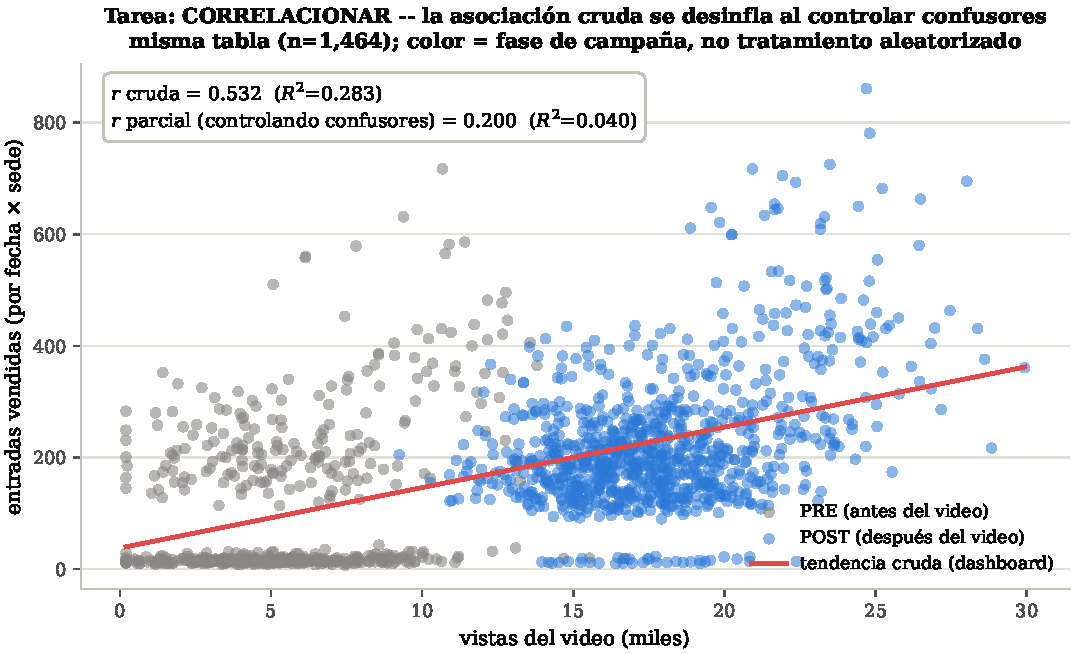
\includegraphics[width=0.85\linewidth]{caso5_q3_scatter.pdf}\caption{La correlación cruda vistas$\leftrightarrow$entradas ($r=0.532$) se desinfla a $r=0.200$ al controlar los confusores compartidos: asociación, no causa \citep{anscombe1973graphs}.}\label{fig:c5-q3}\end{figure}

\paragraph{Decisión.} Cada \emph{story point} declara sus 4 piezas (título analítico, tipo de gráfico, evidencia mínima, mensaje/decisión) y ninguno afirma causalidad; el punto 3 se mantiene como contraevidencia obligatoria antes de llegar a la acción del punto 5.

\paragraph{Límite / trade-off.} Un storyboard de 5 puntos obliga a resumir; se omiten matices (p.\,ej.\ la heterogeneidad por macrozona) que un analista podría querer explorar aparte. Ese es el costo aceptado de un producto explicativo, ya discutido en la pregunta~1.

\subsection{Pregunta 4 --- Memo y bitácora}\label{ssec:c5-q4}

\begin{quote}
Período: mar-jun 2026, video 15-abr. Métrica: ventas incrementales por sol invertido. Evidencia: +100\% bruto en ventas cae a -13\% al restringir a sedes ya abiertas; el coeficiente post cambia de signo al controlar. Método: comparación intra-sedes-abiertas y regresión controlando apertura de sedes, inversión y promociones. Limitación: datos observacionales, efecto no identificado causalmente; sesgo de selección de sede. Acción: no ampliar la campaña; correr un piloto escalonado por sede. Indicador futuro: ventas incrementales por sol invertido en el piloto, contra umbral S/3/sol con IC95\% que excluya cero. \emph{(86 palabras)}
\end{quote}

\bitacora{%
``El video de Killa disparó las ventas +108\%: hay que ampliar la campaña ya.''%
}{%
Ventas incrementales por sol invertido = (ventas POST $-$ ventas esperadas sin cambio de inversión, promo o apertura) / $\Delta$ inversión publicitaria, sobre \texttt{ventas\_soles} por fecha$\times$sede, período abr--jun 2026 vs.\ línea base mar--abr, segmento = sedes abiertas todo el período, meta $\geq$ S/3 de venta incremental por sol con IC95\% que excluya cero.%
}{%
Al desagregar por \texttt{festival\_abierto\_flag} y correr la regresión con confusores (secc.~\ref{ssec:c5-q2}), la diferencia +100\%/+108\% se convierte en $-12.9$\% (intra-sedes-abiertas) y el coeficiente de \texttt{post} se vuelve negativo en ambos modelos controlados ($-5\,185$ a $-6\,460$ soles).%
}{%
``El aumento bruto se confunde con sedes nuevas, inversión y promos; efecto no identificado.''%
}{%
El comité no debe ampliar la campaña basándose en el titular; debe pedir un piloto escalonado con umbral pre-definido antes de comprometer presupuesto adicional.%
}

\texttt{vistas\_video\_miles} y el ``+108\%'' no son el KPI decisor: la primera es una métrica de \textbf{actividad} (exposición, sube $\times3.25$ junto con todo lo demás) y la segunda es un \textbf{resultado} bruto (entradas vendidas sin descontar causas); ninguna conecta el gasto en campaña con un efecto atribuible. Ambas suben porque el tiempo avanza y los confusores --sedes, inversión, promos-- suben con ellas; su correlación con las ventas es en gran parte compartida y \textbf{no identificable como causal} ($R^2$ cruda 0.283 $\to$ $R^2$ parcial $\sim$0.040 al controlar, secc.~\ref{ssec:c5-q3}). El KPI decisor debe ser la métrica de \textbf{impacto} --ventas incrementales por sol invertido, medida con un diseño que separe el video de sus confusores-- porque es la única que responde si vale la pena poner más dinero en la campaña.


% ======================= CONCLUSIONES =======================
\section{Conclusiones}

Los cinco casos comparten una misma moraleja operativa: antes de leer la magnitud hay que fijar el \emph{marco de medición}. En el Caso~1 el marco es el \textbf{denominador} (un promedio ponderado no es el promedio de los ratios de fila); en el Caso~3 es la \textbf{ventana temporal} (doce días no se comparan con treinta y uno); en el Caso~4 es la \textbf{normalización} (volumen y tasa poblacional responden preguntas distintas); en los Casos~2 y~5 es la \textbf{estructura causal} (una asociación observacional, por fuerte que sea su $R^2$, no identifica un efecto sin control de confusores). En todos, el canal perceptual elegido —ángulo de una torta, área de una burbuja, doce colores superpuestos— puede sostener o desmentir la historia con el mismo dato \citep{cleveland1984graphical,munzner2014visualization}. La auditoría no consiste en desconfiar de los números, sino en declarar el marco que los vuelve interpretables y elegir la vista cuya tarea coincide con la decisión.

\begin{thebibliography}{10}
\bibitem[Anscombe(1973)]{anscombe1973graphs} Anscombe, F. J. (1973). Graphs in statistical analysis. \emph{The American Statistician, 27}(1), 17--21.
\bibitem[Cleveland \& McGill(1984)]{cleveland1984graphical} Cleveland, W. S., \& McGill, R. (1984). Graphical perception: Theory, experimentation, and application to the development of graphical methods. \emph{Journal of the American Statistical Association, 79}(387), 531--554.
\bibitem[Few(2009)]{few2009now} Few, S. (2009). \emph{Now You See It: Simple Visualization Techniques for Quantitative Analysis}. Analytics Press.
\bibitem[Gelman(2007)]{gelman2007average} Gelman, A. (2007). Struggles with survey weighting and regression modeling. \emph{Statistical Science, 22}(2), 153--164.
\bibitem[Healy(2018)]{healy2018data} Healy, K. (2018). \emph{Data Visualization: A Practical Introduction}. Princeton University Press.
\bibitem[Munzner(2014)]{munzner2014visualization} Munzner, T. (2014). \emph{Visualization Analysis and Design}. CRC Press.
\bibitem[Simpson(1951)]{simpson1951interpretation} Simpson, E. H. (1951). The interpretation of interaction in contingency tables. \emph{Journal of the Royal Statistical Society: Series B, 13}(2), 238--241.
\bibitem[Tufte(2001)]{tufte2001visual} Tufte, E. R. (2001). \emph{The Visual Display of Quantitative Information} (2nd ed.). Graphics Press.
\bibitem[Wickham(2016)]{wickham2016ggplot2} Wickham, H. (2016). \emph{ggplot2: Elegant Graphics for Data Analysis} (2nd ed.). Springer.
\bibitem[Wilkinson(2005)]{wilkinson2005grammar} Wilkinson, L. (2005). \emph{The Grammar of Graphics} (2nd ed.). Springer.
\end{thebibliography}

\end{document}
